\documentclass[pdflatex,sn-mathphys-num]{sn-jnl}

\usepackage{graphicx}
\usepackage{multirow}
\usepackage{amsmath,amssymb,amsfonts}
\usepackage{amsthm}
\usepackage{mathrsfs}
\usepackage[title]{appendix}
\usepackage{xcolor}
\usepackage{textcomp}
\usepackage{manyfoot}
\usepackage{booktabs}
\usepackage{array}
\usepackage{algorithm}
\usepackage{algorithmicx}
\usepackage{algpseudocode}
\usepackage{listings}
\usepackage{tikz}
\usetikzlibrary{positioning,arrows.meta,fit,shapes.geometric,backgrounds}
\graphicspath{{./}{figures/}}

\raggedbottom

% Numbers of the multi-language replication, written by pilot/v4/paper_v4.py (do not edit by hand)
%% v4-macros: begin
\newcommand{\vNrepos}{14}
\newcommand{\vNchanges}{239}
\newcommand{\vNtest}{144}
\newcommand{\vNcalib}{95}
\newcommand{\vReposGo}{3}
\newcommand{\vChangesGo}{55}
\newcommand{\vTestGo}{33}
\newcommand{\vReposRust}{5}
\newcommand{\vChangesRust}{96}
\newcommand{\vTestRust}{58}
\newcommand{\vReposJSTS}{6}
\newcommand{\vChangesJSTS}{88}
\newcommand{\vTestJSTS}{53}
\newcommand{\vJavaRepos}{3}
\newcommand{\vJavaChanges}{14}
\newcommand{\vJavaTest}{9}
\newcommand{\vJavaCalib}{5}
\newcommand{\vMinChanges}{20}
\newcommand{\vFileMiss}{0.0}
\newcommand{\vFileSaved}{65.3}
\newcommand{\vLineMiss}{6.2}
\newcommand{\vLineSaved}{75.4}
\newcommand{\vStaticMiss}{31.2}
\newcommand{\vNameMiss}{49.3}
\newcommand{\vCrcStaticMiss}{4.2}
\newcommand{\vCrcStaticSaved}{74.1}
\newcommand{\vCrcStaticFiveMiss}{2.1}
\newcommand{\vCrcStaticTwentyMiss}{42.4}
\newcommand{\vMinLambdaTwenty}{0.98}
\newcommand{\vCrcStaticTwentyTestRed}{90.7}
\newcommand{\vCrcStaticTwentyMissGo}{9.1}
\newcommand{\vCrcStaticTwentyMissRust}{31.0}
\newcommand{\vCrcStaticTwentyMissJSTS}{75.5}
\newcommand{\vAciFiveMiss}{4.2}
\newcommand{\vAciFiveSaved}{68.1}
\newcommand{\vWinFiveMiss}{2.8}
\newcommand{\vAciTenMiss}{8.3}
\newcommand{\vAciTenSaved}{75.1}
\newcommand{\vWinTenMiss}{5.6}
\newcommand{\vAciTwentyMiss}{17.4}
\newcommand{\vAciTwentySaved}{76.8}
\newcommand{\vWinTwentyMiss}{25.0}
\newcommand{\vRiskAbMiss}{3.5}
\newcommand{\vRiskAbSaved}{67.2}
\newcommand{\vRiskAbRate}{31.9}
\newcommand{\vLineAbMiss}{1.4}
\newcommand{\vLineAbSaved}{70.3}
\newcommand{\vAciTenMissGo}{9.1}
\newcommand{\vAciFiveMissGo}{6.1}
\newcommand{\vAciTwentyMissGo}{18.2}
\newcommand{\vLineUnsafeNGo}{2}
\newcommand{\vLineMissGo}{6.1}
\newcommand{\vFileSavedGo}{61.9}
\newcommand{\vStaticMissGo}{0.0}
\newcommand{\vAciTenMissRust}{8.6}
\newcommand{\vAciFiveMissRust}{3.4}
\newcommand{\vAciTwentyMissRust}{15.5}
\newcommand{\vLineUnsafeNRust}{5}
\newcommand{\vLineMissRust}{8.6}
\newcommand{\vFileSavedRust}{87.5}
\newcommand{\vStaticMissRust}{29.3}
\newcommand{\vAciTenMissJSTS}{7.5}
\newcommand{\vAciFiveMissJSTS}{3.8}
\newcommand{\vAciTwentyMissJSTS}{18.9}
\newcommand{\vLineUnsafeNJSTS}{2}
\newcommand{\vLineMissJSTS}{3.8}
\newcommand{\vFileSavedJSTS}{43.1}
\newcommand{\vStaticMissJSTS}{52.8}
\newcommand{\vJavaLineMiss}{0.0}
\newcommand{\vJavaFileSaved}{31.3}
\newcommand{\vJavaLineSaved}{63.6}
\newcommand{\vJavaFeasible}{yes}
\newcommand{\vJavaAciTwentyMiss}{11.1}
\newcommand{\vJavaAciTwentySaved}{73.9}
\newcommand{\vJavaAciTwentyMissN}{1}
\newcommand{\vBudgetLearned}{0.866}
\newcommand{\vBudgetCoverage}{0.864}
\newcommand{\vBudgetP}{0.47}
\newcommand{\vBudgetRandom}{0.652}
\newcommand{\vUnsafe}{9}
\newcommand{\vSafe}{135}
\newcommand{\vTrigFileFlag}{8}
\newcommand{\vTrigFileSafePct}{77.0}
\newcommand{\vTrigLineFlag}{8}
\newcommand{\vTrigLineSafePct}{62.2}
\newcommand{\vTrigRiskFlag}{2}
\newcommand{\vTrigRiskSafePct}{28.9}
\newcommand{\vUnsafeGo}{2}
\newcommand{\vTrigRiskFlagGo}{0}
\newcommand{\vUnsafeRust}{5}
\newcommand{\vTrigRiskFlagRust}{0}
\newcommand{\vUnsafeJSTS}{2}
\newcommand{\vTrigRiskFlagJSTS}{2}
\newcommand{\vPyFileOnlyRate}{16.5}
\newcommand{\vPyFileOnlyRateNoImport}{14.9}
\newcommand{\vFileOnlyRateGo}{1.8}
\newcommand{\vFileOnlyRateRust}{5.8}
\newcommand{\vFileOnlyRateJSTS}{9.0}
\newcommand{\vGoRustMaxMissedP}{0.018}
\newcommand{\vGoRustMaxR}{0.083}
\newcommand{\vJSMissedP}{0.197}
\newcommand{\vRustNoStaticPath}{5}
\newcommand{\vQObserved}{8.3}
\newcommand{\vQPredicted}{10.4}
\newcommand{\vProdPredicted}{17.5}
\newcommand{\vQBrier}{0.065}
\newcommand{\vProdBrier}{0.118}
\newcommand{\vConstBrier}{0.076}
\newcommand{\vQPredictedGo}{13.1}
\newcommand{\vProdPredictedGo}{16.7}
\newcommand{\vQObservedGo}{9.1}
\newcommand{\vQPredictedRust}{2.9}
\newcommand{\vProdPredictedRust}{3.8}
\newcommand{\vQObservedRust}{8.6}
\newcommand{\vQPredictedJSTS}{17.0}
\newcommand{\vProdPredictedJSTS}{33.1}
\newcommand{\vQObservedJSTS}{7.5}
\newcommand{\vRRuleAbst}{34.7}
\newcommand{\vRRuleMissProc}{3.2}
\newcommand{\vRRuleSaved}{66.6}
\newcommand{\vRRuleWorst}{6.7}
\newcommand{\vRRuleWorstLang}{Go}
\newcommand{\vQRuleAbst}{29.9}
\newcommand{\vQRuleMissProc}{4.0}
\newcommand{\vQRuleSaved}{66.3}
\newcommand{\vQRuleWorst}{6.7}
\newcommand{\vQRuleWorstLang}{Go}
\newcommand{\vSelRuleAbst}{5.6}
\newcommand{\vSelRuleMissProc}{5.1}
\newcommand{\vSelRuleSaved}{73.7}
\newcommand{\vSelRuleWorst}{6.2}
\newcommand{\vSelRuleWorstLang}{Go}
%% v4-macros: end

\begin{document}

\title[CodeTwin AI: Risk-Calibrated Regression Test Selection]{CodeTwin AI: Evidence-Aware, Risk-Calibrated Regression Test Selection with Abstention---A Survey and a Multi-Language Empirical Study}

\author*[1]{\fnm{Arya} \sur{Godbole}}\email{aaryagodbole550@gmail.com}
\author[1]{\fnm{Suhani} \sur{Bhati}}\email{bhatisuhani5@gmail.com}
\author[1]{\fnm{Madhura} \sur{Suryawanshi}}\email{suryawanshimadhura51@gmail.com}
\author[1]{\fnm{Shreya} \sur{Gole}}\email{shreyakgole@gmail.com}
\author[1]{\fnm{T. A.} \sur{Kamble}}\email{tulsiram17@gmail.com}

\affil[1]{\orgdiv{Department of Computer Science and Engineering (Data Science)}, \orgname{TSSM's Padmabhooshan Vasantdada Patil Institute of Technology}, \orgaddress{\city{Pune}, \state{Maharashtra}, \country{India}}}

\abstract{\textbf{Purpose:} Regression test selection runs only the tests a change may affect but does not say how much risk it leaves. We ask whether selection can keep the share of changes that miss an affected test at a chosen target and flag changes on which conventional selection fails. \textbf{Methods:} We surveyed 32 works, derived requirements from their gaps and designed CodeTwin AI, which ranks tests with a learned model, estimates the residual risk of a selection, calibrates it with conformal risk control and abstains to a broader run when the risk is too high. We evaluated a research prototype of its core on 681 changes of 8 open-source Python projects with three ground truths (including 812 detected seeded faults) and on \vNchanges{} pull requests of \vNrepos{} Go, Rust and JavaScript/TypeScript projects. \textbf{Results:} A threshold fitted once on older commits missed 17.5\% of later changes at a 10\% target, while adaptive conformal inference kept the miss rate at 4.5\%, 9.3\% and 19.9\% for targets of 5\%, 10\% and 20\%. Abstaining on high risk caught 26 of the 31 changes on which line-coverage selection was unsafe, against 7 for rule-based triggers. A change-level risk model was better calibrated than the per-test product formula. In the other languages adaptive calibration held every pooled target, but risk-based abstention caught only \vTrigRiskFlag{} of \vUnsafe{} unsafe changes. \textbf{Conclusion:} Selection can state a calibrated residual risk if calibration adapts over time, and abstaining on that risk helped in Python but not in the other languages.}

\keywords{abstention, adaptive conformal inference, change impact analysis, conformal risk control, mutation testing, regression test selection}

\maketitle

\section{Introduction}\label{sec:intro}
% =====================================================================

Any change to a program can break something that used to work, and regression testing is how developers find out~\cite{yoo2012survey}. On large projects, running the whole suite after every change slows developers down and loads continuous integration (CI)~\cite{elbaum2014ci,memon2017taming}. Regression test selection (RTS) runs only the tests a change can affect, and a selection is \emph{safe} when it keeps all of them~\cite{legunsen2016static}. Mature techniques exist for Java~\cite{gligoric2015ekstazi,liu2023finerts,zhang2024jcgeks}. Python is harder, because importing a module runs code and dynamic features hide where a call goes, yet NameRTS made selection safe on almost every commit it was evaluated on~\cite{wang2026namerts}. Predictive test selection (PTS) learns from past results instead~\cite{machalica2019pts}. AI coding assistants raise the stakes, since they write patches faster than people can review them. In one preprint an agent introduced fewer regressions once it was told which tests a change might affect~\cite{alonso2026tdad}, which is early evidence from a single setup.

We see four gaps in this work. A good average tells us nothing about the risk left in one selection, and PTS thresholds derived from historical samples are no guarantee for a single commit~\cite{machalica2019pts}. Dependency evidence can be incomplete without anyone being told. NameRTS, for instance, documents limits with \texttt{eval}, library code and callbacks from external libraries~\cite{wang2026namerts}. Weak evidence about a change does not necessarily lead to a wider selection. NameRTS selects all tests when a registry decorator changes~\cite{wang2026namerts}, and PTS may rely on running the whole suite from time to time~\cite{machalica2019pts}. And a test that executes changed code counts as evidence for it even if it would still pass with the code broken~\cite{niedermayr2016will}. Statistics can help with the first three. Conformal risk control bounds the expected miss rate under exchangeability~\cite{angelopoulos2024crc}, and conformal methods already make language models abstain~\cite{yadkori2024abstention} and prioritise tests in CI~\cite{altinisik2026conformal}. As far as we know, no technique combines a calibrated risk, visible dependency limits and a fallback to a broader selection when it is unsure.

Our research question is: \emph{can evidence-aware test selection with calibrated abstention keep the miss rate at a chosen target while running substantially fewer tests than the full suite, and does it flag the changes on which conventional selection fails?} We start with Python and then ask which findings carry over to other languages. To answer the question we reviewed the literature, derived requirements from the gaps we found (Sections~\ref{sec:related} and~\ref{sec:requirements}) and designed CodeTwin AI to meet them. We did not build the whole design. The research prototype covers its core, which selects tests, estimates and calibrates their residual risk and abstains, and we compared it with established baselines on the commit histories of Python projects and on pull requests in Go, Rust and JavaScript/TypeScript. Each decision uses only what was known before the change.

The project has five objectives: (O1)~build an evidence graph that shows how files, functions, tests and other repositories are connected and how each link was found; (O2)~select tests by risk within a time budget; (O3)~estimate the risk that remains in a selection, calibrate it to a target miss rate and abstain when the evidence is insufficient; (O4)~integrate with the developer workflow and with AI coding agents; and (O5)~evaluate the result against established baselines on public projects. This paper addresses only part of them. The prototype implements the evidence collection of O1 and the selection, calibration and abstention of O2 and O3 for single repositories, and evaluates them as O5. The rest of O1 (the typed evidence store and evidence from other repositories) and all of O4 are proposed designs, which we describe without evaluating them, so we make no claim about how well they work. For the replication in Section~\ref{sec:rq6} we wrote adapters for Go, Rust, JavaScript/TypeScript and Java. Fig.~\ref{fig:method} shows how the work was carried out and where the evaluated part ends.

\begin{figure}[htbp]
\centering
\resizebox{\linewidth}{!}{%
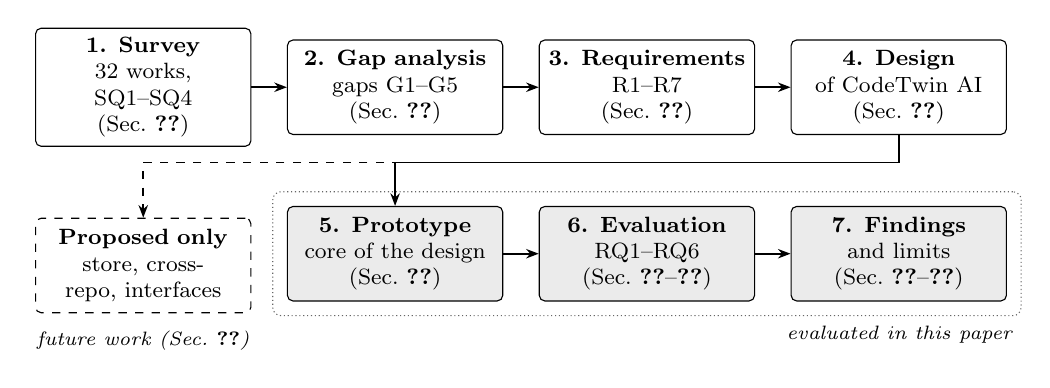
\begin{tikzpicture}[font=\footnotesize, node distance=4mm and 4.5mm,
  st/.style={draw, rounded corners=2pt, align=center, text width=25mm, minimum height=12mm, fill=white},
  ev/.style={st, fill=black!8},
  pr/.style={st, dashed},
  arr/.style={-{Stealth[length=1.6mm]}, semithick}]
\node[st] (s1) {\textbf{1. Survey}\\ 32 works, SQ1--SQ4\\ (Sec.~\ref{sec:related})};
\node[st, right=of s1] (s2) {\textbf{2. Gap analysis}\\ gaps G1--G5\\ (Sec.~\ref{sec:gap})};
\node[st, right=of s2] (s3) {\textbf{3. Requirements}\\ R1--R7\\ (Sec.~\ref{sec:requirements})};
\node[st, right=of s3] (s4) {\textbf{4. Design}\\ of CodeTwin AI\\ (Sec.~\ref{sec:approach})};
\node[pr, below=9mm of s1] (f1) {\textbf{Proposed only}\\ store, cross-repo, interfaces};
\node[ev, below=9mm of s2] (e1) {\textbf{5. Prototype}\\ core of the design\\ (Sec.~\ref{sec:impl})};
\node[ev, below=9mm of s3] (e2) {\textbf{6. Evaluation}\\ RQ1--RQ6\\ (Sec.~\ref{sec:setup}--\ref{sec:results})};
\node[ev, below=9mm of s4] (e3) {\textbf{7. Findings}\\ and limits\\ (Sec.~\ref{sec:discussion}--\ref{sec:threats})};
\draw[arr] (s1) -- (s2); \draw[arr] (s2) -- (s3); \draw[arr] (s3) -- (s4);
\draw[semithick] (s4.south) -- ++(0,-3.5mm) coordinate (h);
\draw[arr] (h) -| (e1.north);
\draw[arr, dashed] (h) -| (f1.north);
\draw[arr] (e1) -- (e2); \draw[arr] (e2) -- (e3);
\begin{scope}[on background layer]
\node[draw=black!60, densely dotted, rounded corners=3pt, inner sep=1.8mm, fit=(e1)(e2)(e3), label={[font=\scriptsize\itshape, anchor=north east]south east:evaluated in this paper}] {};
\end{scope}
\node[font=\scriptsize\itshape, below=1mm of f1] {future work (Sec.~\ref{sec:conclusion})};
\end{tikzpicture}%
}
\caption{How this work was carried out. A survey of 32 works led to five gaps (G1--G5) and seven requirements (R1--R7), from which we designed CodeTwin AI. Only the core of the design, which selects tests, estimates their residual risk, calibrates it and abstains, was built as a research prototype and evaluated on 681 Python changes and \vNchanges{} pull requests in other languages (shaded). The evidence store, cross-repository evidence and the developer and agent interfaces are proposed and left to future work (dashed).}
\label{fig:method}
\end{figure}


The paper makes four contributions.
\begin{itemize}
    \item A targeted survey of 32 works, which shows that efficient selection and a known residual risk have so far been studied separately (Section~\ref{sec:related}), and a design derived from its gaps (Section~\ref{sec:approach}).
    \item A research prototype of the design's core. It treats unresolved dependencies as uncertainty, estimates the residual risk $r(c)$ of each selection, calibrates its threshold with conformal risk control that adapts to drift and abstains to a broader run when the risk is too high. Two change-level additions go with it, a risk model $q(c)$ learned on whole selections and an analysis that finds semantic no-ops, unchecked changed lines and self-confirming tests (Sections~\ref{sec:approach} and~\ref{sec:impl}).
    \item An evaluation on 681 changes of 8 Python projects against ten baselines, with three ground truths: per-test coverage, 812 seeded faults and, on 3 projects, the published ground truth of NameRTS. A replication on \vNtest{} test changes of \vNrepos{} Go, Rust and JavaScript/TypeScript projects shows which findings carry over (Sections~\ref{sec:setup} and~\ref{sec:results}).
    \item A replication package on Zenodo with the scripts, workflows and collected data, from which every reported number is regenerated.
\end{itemize}

% =====================================================================
\section{Background and motivating example}\label{sec:background}
% =====================================================================
\subsection{Key concepts}
Unlike RTS, \textit{test prioritisation} only reorders the tests and never drops one~\cite{yoo2012survey}. Finding the relevant tests requires \textit{change impact analysis}, which can be \textit{static}, reading the code, or \textit{dynamic}, observing it run. Static analysis cannot follow calls through \texttt{getattr} or \texttt{importlib}, and dynamic analysis sees only the paths that ran. \textit{Per-test coverage} records the lines each test runs.

We define the \textit{miss rate} as the fraction of changes on which at least one test that should have run was left out. A risk estimate is \textit{calibrated} if changes estimated as 5\% risky are missed about 5\% of the time. \textit{Conformal risk control} finds a threshold on held-out data that keeps the expected miss rate below a target~\cite{angelopoulos2024crc}, provided calibration and future changes are exchangeable, which commits in time order need not be. \textit{Adaptive conformal inference} (ACI) therefore adjusts the level after each observed error, so that the long-run error rate follows the target under drift~\cite{gibbs2021aci}. \textit{Abstention} means that a system admits it is unsure~\cite{yadkori2024abstention}. Here it then asks for more tests. \textit{Mutation testing} seeds small faults (mutants), and a test kills a mutant if it fails on it, a common proxy for fault detection~\cite{jia2011mutation,just2014mutants}. Code that tests execute but would not notice breaking is \textit{covered but unchecked}, or pseudo-tested for whole methods~\cite{niedermayr2016will}. A \textit{semantic no-op} is a change that cannot alter what the program does, such as an edit to comments or formatting.
\subsection{Motivating example}
Fig.~\ref{fig:example} shows a small scenario. A pull request renames the field \texttt{price} of \texttt{orders.Order} in a shared library, and all of the library's tests pass. Four pieces of code depend on the field. \texttt{billing.total()} calls it statically, \texttt{vendor\_portal/pricing.py} in another repository uses it through an OpenAPI contract, \texttt{customer\_app/cart.py} is seen only at run time and has no tests, and \texttt{plugins.load()} reaches it through \texttt{getattr}, which static analysis cannot follow. A tool that follows only the static and declared links selects two tests and reports the change as ``verified''. The full design of CodeTwin AI would also point out the untested consumer and the unresolved call, report the risk they leave (here above a 5\% target) and suggest running more tests. The prototype we evaluate covers only the single-repository part of this, the static links, coverage and unresolved calls.

\begin{figure}[htbp]
\centerline{\includegraphics[width=\linewidth]{figures/example.png}}
\caption{Impact map for renaming \texttt{orders.Order.price} (red), an illustrative scenario for the full design. Line style shows how each link was found: static analysis (AST), a declared OpenAPI contract, runtime observation, or unresolved (dotted). Green nodes are the selected tests, the orange node is a consumer with no tests, and the dashed node, \texttt{plugins.load()}, uses \texttt{getattr}, so its target is unknown.}
\label{fig:example}
\end{figure}

% =====================================================================
\section{Related work}\label{sec:related}
% =====================================================================
The requirements of CodeTwin AI (Section~\ref{sec:requirements}) come from this review.

\subsection{Survey method}\label{sec:surveymethod}
The review was targeted. We wanted the work closest to our problem rather than a count of every paper on regression testing, and we did not record the number of hits per query. Four survey questions guided the search.
\begin{itemize}
\item SQ1. What evidence do regression test selection techniques use to decide which tests to skip, for which languages and at which granularity?
\item SQ2. Do they report the risk that a selection leaves for an individual change, and what do they do with dependencies they cannot resolve?
\item SQ3. Which statistical methods give calibrated guarantees or let a model abstain, and have they been applied to testing or to code?
\item SQ4. What support exists for AI coding agents to check that a change does not break existing behaviour?
\end{itemize}

\textit{Sources and search terms.} We searched Google Scholar, arXiv, the ACM Digital Library and IEEE Xplore, mainly for papers published at ISSTA, ASE, ICSE, FSE and ICLR between 2015 and 2026, and added earlier foundational studies. Each search paired a topic with a qualifier. We combined ``regression test selection'' with ``safety'', ``Python'', ``multi-language'', ``machine learning'' or ``continuous integration'', and ``change impact analysis'' with ``survey'' or ``call graph''. For the statistical side we paired ``conformal prediction'' or ``conformal risk control'' with ``selection'', ``software'' or ``defect prediction'', and searched for ``selective classification'' and ``abstention''. For agents we combined ``coding agent'' with ``regression'', ``test'' or ``SWE-bench''. We also went through the related work of the closest papers (NameRTS, Ekstazi, conformal risk control and TDAD) for further candidates.

\textit{Inclusion and exclusion.} A work was included if it proposes or evaluates a technique for test selection, test prioritisation, change impact analysis or test adequacy, a calibration or abstention method that could carry over to such decisions, or testing support for AI coding agents, provided it also reports an empirical evaluation or is a widely cited foundation. We left out tool documentation, blog posts and works whose full text we could not read. Recent preprints were included when they were the only source on a topic.

\textit{Data extraction.} For every work we noted the approach, the evaluation (subjects and size), the main quantitative finding and its limitation for our problem (Tables~S1 and~S2 in Online Resource~1). For selection techniques we also noted the language, the kind of evidence, the level at which dependencies are tracked and what the technique returns (Table~\ref{tab:taxonomy}).

We kept 32 works that are either foundational or close to our problem, without aiming at exhaustive coverage. Online Resource~1 summarises each of them (Tables~S1 and~S2), and the subsections below group them by theme, together with some related works that are not in the tables.


\subsection{Foundations and precise selection}
Yoo and Harman~\cite{yoo2012survey} separate test-suite minimisation, regression test selection and test prioritisation, and Rothermel and Harrold~\cite{rothermel1996analyzing} compare selection techniques by inclusiveness (a fully inclusive technique is safe), precision, efficiency and generality. Selection rests on change impact analysis, whose code-based techniques Li et al.\ surveyed~\cite{li2013cia}. Ekstazi reruns a test only when a file it used at run time changes, and on 615 revisions of 32 projects it cut testing time by 32\% on average~\cite{gligoric2015ekstazi}. Static class-level selection did about as well but was sometimes unsafe~\cite{legunsen2016static}, and STARTS implements it as a Maven tool that needs neither instrumentation nor a test run~\cite{legunsen2017starts}. Later work refines the dependencies. FineEkstazi and FineSTARTS show that some semantics-modifying changes do not require rerunning the tests they affect~\cite{liu2023finerts}, JcgEks adds static method call graphs to Ekstazi's file dependencies~\cite{zhang2024jcgeks}, and HyRTS mixes method and file granularity~\cite{zhang2018hyrts}. Reks skips tests affected only by behaviour-preserving refactorings~\cite{wang2018reks}, TASTING reuses results while the syntax trees a test reaches are unchanged~\cite{landsberg2022tasting}, and reflection-aware selection keeps static selection safe under Java reflection, although it resolves such calls without reporting them~\cite{shi2019reflection}. Selection across languages works either below the language, as RTSLinux and the system-call tracing of Elsner et al.\ do~\cite{celik2017jvm,elsner2022multilang,elsner2023binaryrts}, or with small per-language descriptions, as in BabelRTS~\cite{maurina2025babelrts}. Our adapters borrow that last idea. Every one of these evaluations reports safety and savings as averages over changes.

\subsection{Coverage, Python and learned selection}
Coverage drives prioritisation~\cite{rothermel2001prioritizing} and is used at scale at Google~\cite{ivankovic2019coverage}. iJaCoCo keeps it current cheaply~\cite{wang2024ijacoco}, and tree kernels over syntax trees measure how much a change alters the code in order to prioritise tests~\cite{altiero2024treekernel}. Covered code is not necessarily checked code. When Niedermayr et al.\ emptied covered methods, the covering tests often still passed~\cite{niedermayr2016will}, and statements that run without any assertion depending on them made up 5\% to 39\% of covered statements in a later study~\cite{maton2025oracle}.

For Python, PyCG's static call graphs reached about 69.9\% recall on real packages~\cite{salis2021pycg}, so a selection built on them would silently treat roughly one real edge in three as no dependency. NameRTS avoids call graphs and matches names instead. On 500 commits of ten projects it skipped 69.9\% of test files and kept all affected tests on 99.6\% of commits~\cite{wang2026namerts}, but its answer is still yes or no. With coverage-based selection on three Python projects, Kauhanen et al.\ missed 0--2\% of seeded faults at file level and 16--24\% at line level~\cite{kauhanen2021python}, and pytest-ranking reorders pytest suites to find failures sooner~\cite{cheng2025pytestranking}.

Learned selection replaces explicit dependencies with a model. Predictive test selection at Meta caught more than 99.9\% of faulty changes while halving the infrastructure cost of testing, but its threshold comes from historical samples and gives no guarantee for one change~\cite{machalica2019pts}. Other work compares learning approaches in CI~\cite{bertolino2020learning}, uses co-evolution of tests and code as the relevance label~\cite{jungwirth2026pto}, generates tests with language models~\cite{foster2025ach} or finds that simple heuristics compete with learned models~\cite{elsner2021readily}.

\subsection{Calibration, abstention and AI coding agents}
Selective classification lets a model reject inputs so that its error on the rest stays at a chosen level~\cite{geifman2017selective}. Conformal methods give such guarantees without assuming a particular distribution, provided the data are exchangeable~\cite{angelopoulos2023gentle}, and conformal risk control bounds the expected value of a monotone loss such as the miss rate, assuming exchangeability~\cite{angelopoulos2024crc}. Selective conformal risk control adds an abstention step for classification~\cite{xu2026scrc}, and conformal selection controls the false discovery rate when picking promising candidates~\cite{jin2023selection}. Test selection asks the opposite question, which tests may be left out. Conformal methods have reached testing and code, in a per-test run-or-skip prototype with ACI~\cite{crcpts2026}, in conformal prioritisation in CI~\cite{altinisik2026conformal} and in just-in-time defect prediction~\cite{shahini2024jitcp}, and they make language models abstain instead of hallucinating~\cite{yadkori2024abstention}.

AI coding agents make this a practical problem. SWE-bench collects real issues from Python repositories~\cite{jimenez2024swebench}, and language models still build less complete call graphs than PyCG~\cite{venkatesh2025llmcg}. TDAD gives an agent a static map from code to tests and lowered its regression rate from 6.08\% to 1.82\% on 100 SWE-bench Verified instances~\cite{alonso2026tdad}, yet the map has no confidence attached. In 64.8\% of the Python pull requests written by agents in one study, no existing test executed a changed line~\cite{dipongkor2026agentic}. ExecCritic checks that an agent's regression test fails before the fix~\cite{tao2026execcritic}, GTDD adds adversarial inputs~\cite{kato2026gtdd}, and a repair agent at Google was made to skip bugs it was unlikely to fix~\cite{cambronero2026abstain}, but on the judgement of a language model and without a statistical guarantee.

\subsection{Summary and research gap}\label{sec:gap}
\textit{Answers to the survey questions.} For SQ1, selection techniques draw on four kinds of evidence: static dependencies (STARTS, BabelRTS), dynamic dependencies recorded while tests run (Ekstazi, RTSLinux and the work of Elsner et al.), names (NameRTS) and learned failure histories (predictive test selection). Most of them track dependencies at file or class level, most were built for Java, and the few that span languages work on files (Table~\ref{tab:taxonomy}). For SQ2, none of the reviewed selection techniques reports the risk left for an individual change. Dependencies they cannot resolve are either dropped, as happens to missing call-graph edges~\cite{salis2021pycg}, or handled by selecting everything in a known risky case, as NameRTS does when a registry decorator changes~\cite{wang2026namerts}. For SQ3, selective classification, conformal risk control and its selective variant, adaptive conformal inference and conformal selection all give guarantees or allow abstention~\cite{geifman2017selective,angelopoulos2024crc,xu2026scrc,gibbs2021aci,jin2023selection}. In software engineering we found them applied to just-in-time defect prediction, to test prioritisation in CI and to a per-test run-or-skip prototype~\cite{shahini2024jitcp,altinisik2026conformal,crcpts2026}, but never to the risk of the selection for one change. For SQ4, agents receive either a code-to-test map without any confidence~\cite{alonso2026tdad} or abstain on the judgement of a language model~\cite{cambronero2026abstain}, and none of them receives a calibrated signal to stop and run more tests.

\begin{table}[htbp]
\caption{Classification of the reviewed selection techniques}
\label{tab:taxonomy}
\centering
\footnotesize
\setlength{\tabcolsep}{3pt}
\renewcommand{\arraystretch}{1.15}
\begin{tabular}{@{}>{\raggedright\arraybackslash}p{0.17\textwidth}>{\raggedright\arraybackslash}p{0.12\textwidth}>{\raggedright\arraybackslash}p{0.25\textwidth}>{\raggedright\arraybackslash}p{0.14\textwidth}>{\raggedright\arraybackslash}p{0.12\textwidth}>{\raggedright\arraybackslash}p{0.10\textwidth}@{}}
\toprule
\textbf{Technique} & \textbf{Language} & \textbf{Evidence} & \textbf{Dependency level} & \textbf{Returns} & \textbf{Per-change risk} \\
\midrule
Ekstazi~\cite{gligoric2015ekstazi} & Java & Dynamic file dependencies & File & Selection & No \\
STARTS~\cite{legunsen2017starts} & Java & Static class dependencies & Class & Selection & No \\
FineEkstazi, FineSTARTS~\cite{liu2023finerts} & Java & Dynamic or static, with change semantics & Class & Selection & No \\
HyRTS~\cite{zhang2018hyrts} & Java & Dynamic, hybrid & Method and file & Selection & No \\
JcgEks~\cite{zhang2024jcgeks} & Java & Dynamic files plus static call graph & File and method & Selection & No \\
TASTING~\cite{landsberg2022tasting} & C & Hashes of the syntax trees a test reaches & Syntax tree & Reused results & No \\
RTSLinux~\cite{celik2017jvm} & Any (Java evaluated) & Dynamic, operating-system file accesses & File & Selection & No \\
Elsner et al.~\cite{elsner2022multilang} & Java, C/C++ & Dynamic, system-call tracing & File & Selection & No \\
BinaryRTS~\cite{elsner2023binaryrts} & C++ & Dynamic binary instrumentation & Function and external file & Selection & No \\
BabelRTS~\cite{maurina2025babelrts} & Many & Static, per-language patterns & File & Selection & No \\
NameRTS~\cite{wang2026namerts} & Python & Static names plus run-time probing & Code element & Selection & No \\
Kauhanen et al.~\cite{kauhanen2021python} & Python & Dynamic coverage & File or line & Selection & No \\
Predictive test selection~\cite{machalica2019pts} & Any & Learned from test history & Change--test pair & Selection & Aggregate \\
Conformal CI ranking~\cite{altinisik2026conformal} & Java & History plus adaptive conformal calibration & Test & Ranked candidate set & No \\
TDAD~\cite{alonso2026tdad} & Python & Static code-to-test map & Test & Map for an agent & No \\
\textbf{CodeTwin AI prototype} & Python (Go, Rust, JS/TS, Java in RQ6) & Previous coverage, static facts, learned and calibrated & Test file & Selection, $r(c)$, $q(c)$, abstention & Yes \\
\bottomrule
\end{tabular}
\end{table}

\textit{Gaps.} Table~\ref{tab:gap} compares the closest work with CodeTwin AI by language, multi-repository support, a risk estimate for an individual change, calibrated abstention and blind-spot reporting. The answers to the survey questions leave five gaps, G1 to G5, which Section~\ref{sec:requirements} turns into requirements.
\begin{enumerate}
\item G1 (no per-change risk). Techniques report safety as an average over many commits, NameRTS included~\cite{wang2026namerts}, and nothing tells the developer how risky an individual change is.
\item G2 (hidden blind spots). Calls that static analysis cannot resolve, such as those made through \texttt{getattr}, are dropped without the developer being told~\cite{salis2021pycg}.
\item G3 (no fallback when evidence is weak). The methods to calibrate and abstain exist (SQ3), but no technique we found selects tests for a single change with an explicit risk and the option to abstain.
\item G4 (one language, one repository). The semantics-aware and hybrid selectors target only Java~\cite{liu2023finerts,zhang2024jcgeks} and NameRTS targets Python~\cite{wang2026namerts}, and none of the reviewed techniques follows dependants into other repositories.
\item G5 (coverage taken as checking). Coverage is taken as evidence that a change is tested, although a covering test may not notice a fault in the covered code~\cite{niedermayr2016will}, and none of the selection techniques we reviewed weakens its evidence for that reason.
\end{enumerate}
Taken together, we could not find a technique that combines a residual-risk estimate for an individual change, calibration against a desired miss rate, abstention and explicit reporting of blind spots. Because our search was not exhaustive, we do not claim that no such work exists.
\begin{table}[htbp]
\caption{Comparison of the closest work with CodeTwin AI}
\label{tab:gap}
\centering
\footnotesize
\setlength{\tabcolsep}{1.8pt}
\begin{tabular}{@{}lccccc@{}}
\toprule
\textbf{Work} & \textbf{Lang.} & \textbf{Multi-repo} & \textbf{Risk} & \textbf{Abstain} & \textbf{Blind spots} \\
\midrule
NameRTS & Python & No & No & No & No \\
Predictive Test Sel. & Any & No & Aggregate & No & No \\
Conformal CI ranking & Java & No & No & No & No \\
BabelRTS & Many & No & No & No & No \\
TDAD & Python & No & Score & No & No \\
Abstain and Validate & --- & No & No & Model-based & No \\
\textbf{CodeTwin AI} & Python$^{a}$ & Design & Yes & Yes & Yes \\
\bottomrule
\end{tabular}
\par\smallskip\raggedright\footnotesize $^{a}$The prototype is evaluated on Python; the replication in Section~\ref{sec:rq6} adds Go, Rust, JavaScript/TypeScript and Java. ``Design'': part of the proposed design, not of the evaluated prototype.
\end{table}

% =====================================================================
\section{Proposed approach: CodeTwin AI}\label{sec:approach}
% =====================================================================

\subsection{From gaps to requirements}\label{sec:requirements}
Table~\ref{tab:req} traces each gap of Section~\ref{sec:gap} to a requirement, the component meant to meet it, the research question that tests it and how far this paper goes (R7 comes from SQ4). The prototype meets R1, R2 and R4, meets R3, R5 and R6 in part, and leaves R7 as an unevaluated design.

\begin{table}[htbp]
\caption{Requirements derived from the gaps, and how far this paper goes}
\label{tab:req}
\centering
\footnotesize
\setlength{\tabcolsep}{4pt}
\renewcommand{\arraystretch}{1.15}
\begin{tabular}{@{}>{\raggedright\arraybackslash}p{0.05\textwidth}>{\raggedright\arraybackslash}p{0.27\textwidth}>{\raggedright\arraybackslash}p{0.24\textwidth}>{\raggedright\arraybackslash}p{0.07\textwidth}>{\raggedright\arraybackslash}p{0.25\textwidth}@{}}
\toprule
\textbf{Gap} & \textbf{Requirement} & \textbf{Component (Section)} & \textbf{RQ} & \textbf{Status in this paper} \\
\midrule
G1 & R1: estimate the risk that the selection for one change misses an affected test & Residual risk $r(c)$ and change-level risk $q(c)$ (\ref{sec:risk}, \ref{sec:qc}) & RQ2, RQ3 & Prototype; evaluated \\
G1 & R2: keep the miss rate at a target the user chooses, also when the project drifts & Conformal risk control and adaptive conformal inference (\ref{sec:crc}) & RQ2 & Prototype; evaluated \\
G2 & R3: record dependencies the analysis cannot resolve and show them instead of dropping them & Unresolved edges and dynamic-call facts in the evidence graph (\ref{sec:graph}) & RQ3 & Partly: dynamic-call facts evaluated as triggers; evidence store and reports proposed \\
G3 & R4: run a broader set of tests when the evidence for a change is weak & Risk-based abstention and uncertainty triggers (\ref{sec:risk}, \ref{sec:qc}) & RQ3 & Prototype; evaluated \\
G4 & R5: work for other languages and, later, across repositories & Language adapters; cross-repository evidence (\ref{sec:impl}) & RQ6 & Partly: adapters evaluated; cross-repository evidence proposed \\
G5 & R6: weaken evidence from tests that run a change without checking it, or that pass without it & No-op, unchecked-line and self-confirming test analysis (\ref{sec:changeev}) & RQ5 & Partly: measured; discounts in $r(c)$ proposed \\
SQ4 & R7: give developers and AI agents the decision and its evidence before merging & VS Code extension, pull-request check, MCP server (\ref{sec:interfaces}) & --- & Proposed; not evaluated \\
\bottomrule
\end{tabular}
\end{table}

\subsection{Problem formulation}
Let $c$ be a commit that changes some source files of a project with test suite $T$. CodeTwin AI selects whole test files, and the run time $t(i)$ of a test file $i\in T$ is taken from the previous commit or, for a new file, set to the median run time. Let $A(c)\subseteq T$ be the test files that $c$ truly affects (defined in Section~\ref{sec:setup}) and $F(c)\subseteq T$ the test files that $c$ adds or modifies, which always run. For each commit the system returns a subset $S(c)$ with $F(c)\subseteq S(c)$ together with a decision, \textsc{Proceed} or \textsc{Abstain}, where abstaining means running a larger set of tests, either the full suite or a broader evidence-based selection. A commit is \emph{missed} if $A(c)\nsubseteq S(c)$.

The framework has two modes. In \emph{budget mode} the developer fixes a time budget $B$, and the selection must satisfy
\begin{equation}
\textstyle\sum_{i\in S(c)} t(i) \le B . \label{eq:budget}
\end{equation}
In \emph{calibrated mode} the developer instead fixes a target miss rate $\alpha$, and the expected miss rate over future commits must stay at or below it:
\begin{equation}
\mathbb{E}\big[\,\mathbf{1}\{A(c)\nsubseteq S(c)\}\,\big] \le \alpha . \label{eq:risk}
\end{equation}
We call the probability that a selection misses an affected test its \emph{residual risk}, and $r(c)$ is our estimate of it for one change (Section~\ref{sec:risk}). Calibrated mode bounds the miss rate over many changes, whereas abstention acts on the single changes whose estimated risk is too high.

We assume that tests are selected per file (Table~\ref{tab:decisions}), that they are deterministic, so flaky tests are not modelled~\cite{parry2022flaky}, and that the decision for $c$ uses only the diff and static facts of $c$ and the coverage and run times recorded on the previous commit. Since budgets are usually expressed relative to the full suite, we write $B=b\cdot\sum_{i\in T}t(i)$ with $b\in(0,1]$ and report results for $b\in\{0.10,0.25,0.50\}$.

\subsection{Architecture}
Fig.~\ref{fig:arch} shows the four layers of CodeTwin AI. \emph{Layer~1} gathers evidence about a change: changed lines from the git diff, imports and dynamic-call markers from language adapters, per-test coverage and run times from the test runner, declared dependencies from manifests and API contracts and, optionally, suggestions from a local language model. \emph{Layer~2} links this evidence in a graph. \emph{Layer~3} scores every test file, selects tests and abstains when the estimated residual risk exceeds the target. \emph{Layer~4} delivers the decision to developers and, through a Model Context Protocol (MCP) server, to AI coding agents. The prototype implements Layer~3 and most of Layers~1 and~2 (Section~\ref{sec:impl}). The typed evidence store, the language-model suggestions and Layer~4 are designed but not evaluated in this paper.

The analysis runs locally, on the developer's machine or the CI runner, and no code leaves it unless the optional language model is switched on. A new language needs only an adapter that writes evidence in a common format, so everything above Layer~1 is shared. SQLite and NetworkX are enough for the repository sizes we target, so the design needs no graph database.

\begin{figure}[htbp]
\resizebox{\linewidth}{!}{%
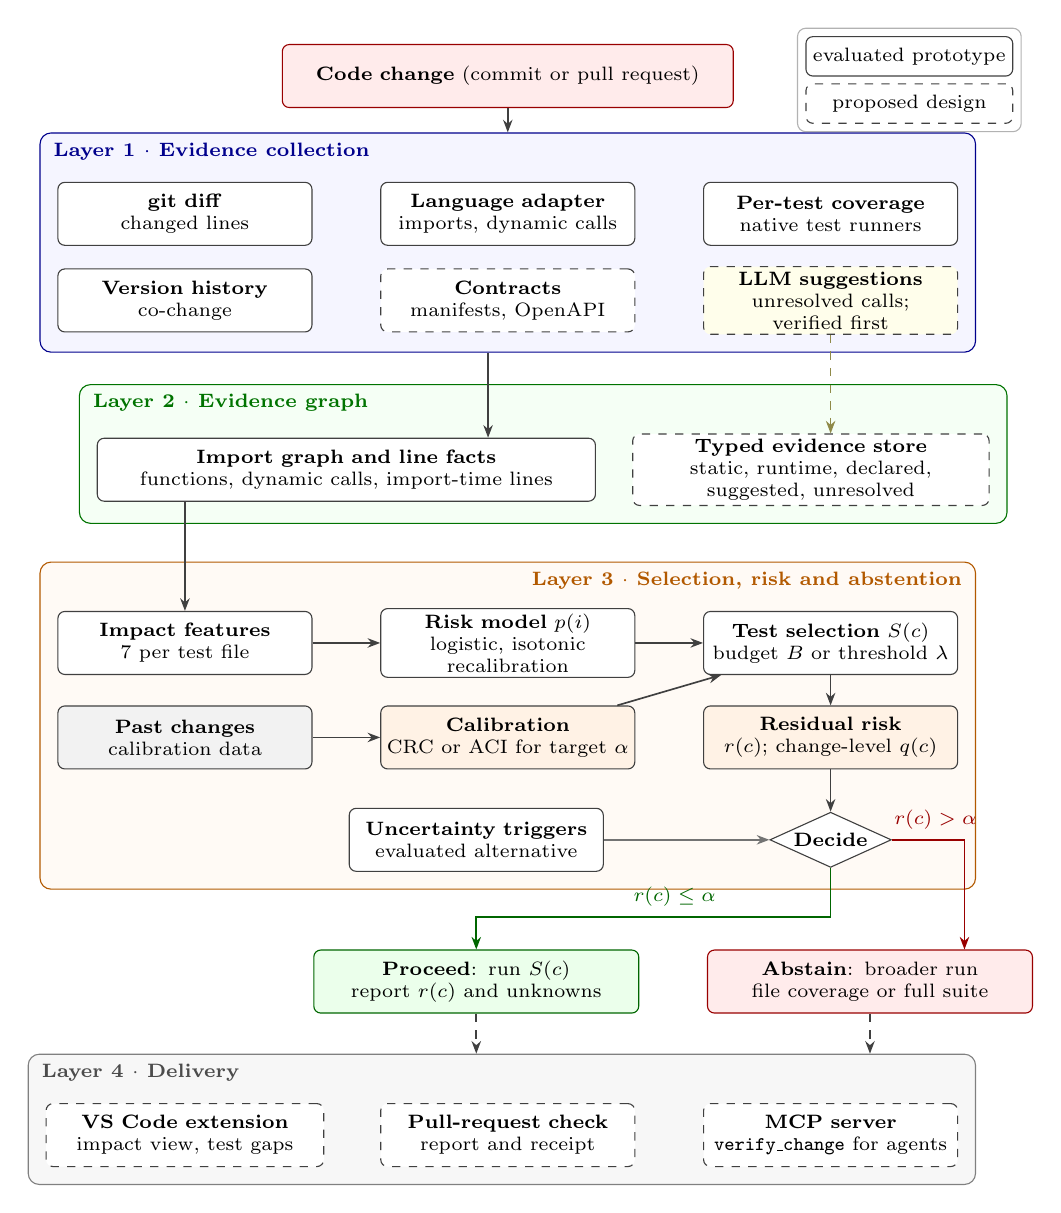
\begin{tikzpicture}[font=\scriptsize,
  b/.style={draw=black!75, rounded corners=2.5pt, align=center, fill=white, minimum height=8mm, inner sep=1.8pt, text width=31mm},
  p/.style={b, dashed},
  lay/.style={draw, rounded corners=4pt, inner sep=2.2mm},
  lt/.style={font=\scriptsize\bfseries, anchor=north west, inner sep=1.5pt},
  ar/.style={-{Stealth[length=1.6mm]}, black!75, semithick}]
% input
\node[b, text width=56mm, fill=red!8, draw=red!60!black] (chg) at (0,0.00) {\textbf{Code change} (commit or pull request)};
\node[b, text width=25mm, minimum height=5mm] (lg1) at (5.1,0.25) {evaluated prototype};
\node[p, text width=25mm, minimum height=5mm] (lg2) at (5.1,-0.35) {proposed design};
% layer 1
\node[b] (diff) at (-4.1,-1.75) {\textbf{git diff}\\ changed lines};
\node[b] (adp)  at (0,-1.75)    {\textbf{Language adapter}\\ imports, dynamic calls};
\node[b] (cov)  at (4.1,-1.75)  {\textbf{Per-test coverage}\\ native test runners};
\node[b] (hst)  at (-4.1,-2.85) {\textbf{Version history}\\ co-change};
\node[p] (con)  at (0,-2.85)    {\textbf{Contracts}\\ manifests, OpenAPI};
\node[p, fill=yellow!8] (llm) at (4.1,-2.85) {\textbf{LLM suggestions}\\ unresolved calls; verified first};
% layer 2
\node[b, text width=62mm] (grf) at (-2.05,-5.00) {\textbf{Import graph and line facts}\\ functions, dynamic calls, import-time lines};
\node[p, text width=44mm] (sto) at (3.85,-5.00) {\textbf{Typed evidence store}\\ static, runtime, declared, suggested, unresolved};
% layer 3
\node[b] (fea) at (-4.1,-7.20) {\textbf{Impact features}\\ 7 per test file};
\node[b] (mod) at (0,-7.20)    {\textbf{Risk model} $p(i)$\\ logistic, isotonic recalibration};
\node[b] (sel) at (4.1,-7.20)  {\textbf{Test selection} $S(c)$\\ budget $B$ or threshold $\lambda$};
\node[b, fill=black!5] (pst) at (-4.1,-8.40) {\textbf{Past changes}\\ calibration data};
\node[b, fill=orange!10] (cal) at (0,-8.40) {\textbf{Calibration}\\ CRC or ACI for target $\alpha$};
\node[b, fill=orange!10] (rsk) at (4.1,-8.40) {\textbf{Residual risk}\\ $r(c)$; change-level $q(c)$};
\node[b] (trg) at (-0.4,-9.70) {\textbf{Uncertainty triggers}\\ evaluated alternative};
\node[draw=black!75, diamond, aspect=2.2, fill=white, inner sep=1pt] (dec) at (4.1,-9.70) {\textbf{Decide}};
% outputs
\node[b, text width=40mm, fill=green!8, draw=green!40!black] (go) at (-0.4,-11.50) {\textbf{Proceed}: run $S(c)$\\ report $r(c)$ and unknowns};
\node[b, text width=40mm, fill=red!8, draw=red!60!black] (ab) at (4.6,-11.50) {\textbf{Abstain}: broader run\\ file coverage or full suite};
% layer 4
\node[p, text width=34mm] (vsc) at (-4.1,-13.45) {\textbf{VS Code extension}\\ impact view, test gaps};
\node[p] (prc) at (0,-13.45)    {\textbf{Pull-request check}\\ report and receipt};
\node[p] (mcp) at (4.1,-13.45)  {\textbf{MCP server}\\ \texttt{verify\_change} for agents};
% layers
\begin{scope}[on background layer]
\node[lay, draw=blue!55!black, fill=blue!4, fit=(diff)(cov)(hst)(llm), inner ysep=4.2mm, yshift=2mm] (L1) {};
\node[lay, draw=green!45!black, fill=green!4, fit=(grf)(sto), inner ysep=4.2mm, yshift=2mm] (L2) {};
\node[lay, draw=orange!70!black, fill=orange!4, fit=(fea)(sel)(pst)(trg)(dec), inner ysep=4.2mm, yshift=2mm] (L3) {};
\node[lay, draw=black!50, fill=black!3, fit=(vsc)(mcp), inner ysep=4.2mm, yshift=2mm] (L4) {};
\node[draw=black!30, rounded corners=3pt, fit=(lg1)(lg2), inner sep=1mm] {};
\end{scope}
\node[lt, text=blue!55!black] at ([shift={(1.2mm,-0.7mm)}]L1.north west) {Layer 1 $\cdot$ Evidence collection};
\node[lt, text=green!45!black] at ([shift={(1.2mm,-0.7mm)}]L2.north west) {Layer 2 $\cdot$ Evidence graph};
\node[lt, text=orange!70!black, anchor=north east] at ([shift={(-1.2mm,-0.7mm)}]L3.north east) {Layer 3 $\cdot$ Selection, risk and abstention};
\node[lt, text=black!70] at ([shift={(1.2mm,-0.7mm)}]L4.north west) {Layer 4 $\cdot$ Delivery};
% arrows
\draw[ar] (chg) -- (L1.north -| chg);
\draw[ar] ([xshift=18mm]L1.south -| grf) -- ([xshift=18mm]grf.north);
\draw[ar, dashed, yellow!50!black] (llm.south) -- (sto.north -| llm.south);
\draw[ar] (grf.south -| fea) -- (fea.north);
\draw[ar] (fea) -- (mod); \draw[ar] (mod) -- (sel);
\draw[ar] (pst) -- (cal); \draw[ar] (cal) -- (sel);
\draw[ar] (sel) -- (rsk); \draw[ar] (rsk) -- (dec);
\draw[ar, black!55] (trg) -- (dec);
\draw[ar, green!40!black] (dec.south) -- ++(0,-0.62) -| node[pos=0.22, above, font=\scriptsize]{$r(c)\le\alpha$} (go.north);
\draw[ar, red!60!black] (dec.east) -| node[pos=0.3, above, font=\scriptsize]{$r(c)>\alpha$} ([xshift=12mm]ab.north);
\draw[ar, dashed] (go.south) -- (L4.north -| go.south);
\draw[ar, dashed] (ab.south) -- (L4.north -| ab.south);
\end{tikzpicture}%
}
\caption{Architecture and decision flow of CodeTwin AI. Layer~1 collects evidence about a change, and Layer~2 links it in a graph: in the prototype an import graph with line-level facts, in the full design a typed evidence store. Layer~3 calculates a score for each test file and selects tests within a budget or above a threshold calibrated on recent commits; if the estimated residual risk is above the target, it abstains to a broader run (rule-based uncertainty triggers are evaluated as an alternative). Layer~4 delivers the decision. Solid boxes are part of the research prototype evaluated in this paper; dashed boxes are proposed designs that this paper does not evaluate. Language adapters (Python: \texttt{ast}, pytest and coverage.py; other languages: tree-sitter and each language's own test runner and coverage tool, Section~\ref{sec:impl}) provide the same evidence, and everything above them is shared.}
\label{fig:arch}
\end{figure}

\subsection{Design decisions and alternatives}\label{sec:decisions}
Table~\ref{tab:decisions} lists the main design questions, the alternatives we considered and the choice made. Where the survey did not settle a question, the prototype implements both alternatives and the evaluation decides.

\begin{table}[htbp]
\caption{Design decisions, alternatives and the choice made in the prototype}
\label{tab:decisions}
\centering
\footnotesize
\setlength{\tabcolsep}{4pt}
\renewcommand{\arraystretch}{1.15}
\begin{tabular}{@{}>{\raggedright\arraybackslash}p{0.15\textwidth}>{\raggedright\arraybackslash}p{0.22\textwidth}>{\raggedright\arraybackslash}p{0.24\textwidth}>{\raggedright\arraybackslash}p{0.30\textwidth}@{}}
\toprule
\textbf{Question} & \textbf{Alternatives} & \textbf{Choice in the prototype} & \textbf{Reason} \\
\midrule
How are tests linked to code? & Static call graph; name matching; per-test coverage & Coverage of the previous version, plus static imports and dynamic-call markers & A static Python call graph missed about 30\% of real call edges~\cite{salis2021pycg}; coverage sees only executed paths, so the static facts mark what it may miss \\
What is selected? & Single test functions; test files & Test files & pytest reports run times per file, and start-up cost would dominate single functions \\
How is a test scored? & Deep model; transparent model & Logistic regression, recalibrated with isotonic regression & Every score can be traced back to its features \\
How is the threshold set? & Fixed once on older commits; adaptive conformal inference & Both, compared in RQ2 & Commits are ordered in time and need not be exchangeable \\
How is the risk of a selection estimated? & Product over skipped tests, $r(c)$; learned per change, $q(c)$ & Both, compared in RQ2 and RQ3 & The product assumes that skipped tests are independent \\
What happens when evidence is weak? & Rule-based triggers; risk-based abstention & Both, compared in RQ3 & Rules are easy to explain; a risk rule adapts to the project \\
What runs after abstaining? & Full suite; file-coverage selection; static reachability plus file coverage & All three, compared in RQ3 & The broader run trades safety against saved time \\
How are other languages added? & A separate tool per language; an adapter with a common evidence format & Adapter & Everything above the evidence layer stays the same for every language \\
\bottomrule
\end{tabular}
\end{table}

\subsection{Blind-spot-aware evidence graph}\label{sec:graph}
In the full design every edge of the graph carries one kind of evidence: \emph{static}, \emph{runtime-observed}, \emph{declared} (from a manifest or API contract), \emph{co-change}, \emph{suggested} by a language model and not yet verified, or \emph{unresolved}. An unresolved edge is one the analysis knows exists but cannot follow, such as a \texttt{getattr} call with a computed name. Such edges are stored and reported, never treated as ``no dependency'', and each record keeps its source, tool and time, so that stale evidence can be recognised.

For every version of every source file the prototype stores three line-level facts: the span of each function including its decorators; the lines with a dynamic call (\texttt{eval}, \texttt{exec}, \texttt{\_\_import\_\_}, \texttt{import\_module}, or \texttt{getattr}/\texttt{setattr}/\texttt{hasattr} with a computed name); and the lines run at import time, that is, module-level and class-level statements other than imports, docstrings and simple constants, plus all decorators. From this evidence it computes seven features for each pair of a change and a test file $i$, using only the coverage of the previous version and the static facts and diff of the new one: (1)~$x_{\mathit{line}}$, whether $i$ executed a changed line; (2)~$x_{\mathit{func}}$, whether $i$ executed the body of a function that encloses a changed line or insertion point; (3)~$x_{\mathit{file}}$, whether $i$ executed any changed file; (4)~$x_{\mathit{imp}}=1/d$, where $d$ is the import distance from $i$ to a changed module (at most six, and $0$ if unreachable); (5)~$x_{\mathit{name}}$, whether the name of $i$ contains the name of a changed module; (6)~$x_{\mathit{co}}$, the share of the last 300 commits touching the changed files that also touched $i$; and (7)~$x_{\mathit{chg}}$, whether $i$ itself was added or changed.

Changed lines come from a zero-context \texttt{git diff} between the evaluated parent and the change. Because the parent's coverage is matched against the \emph{old} line numbers, nothing from running the tests of the change is used. Lines that coverage.py records outside any test context count as import-time lines. The import graph contains every \texttt{import} and \texttt{from}\ldots\texttt{import} statement, with relative imports resolved against the package path.

\subsection{Budgeted, risk-ranked selection}\label{sec:select}
A logistic regression model with balanced class weights predicts how likely it is that test file $i$ is affected:
\begin{equation}
p(i) = \sigma\!\left(\mathbf{w}^{\top}\mathbf{x}_i + b\right), \label{eq:model}
\end{equation}
where $\mathbf{x}_i$ is the feature vector and $\sigma$ the logistic function. In budget mode (Algorithm~\ref{alg:select}, lines 1--7) the tests in $F(c)$ are taken first, and the others follow in descending order of $p(i)/t(i)$, the risk per second, for as long as the budget allows. This is the greedy heuristic for the knapsack problem. In calibrated mode (lines 8--14) every test with $p(i)\ge\hat\lambda_c$ is selected, where $\hat\lambda_c$ is a calibrated threshold (Section~\ref{sec:crc}), unless the system abstains.

\begin{algorithm}[t]
\caption{Risk-ranked selection with calibrated abstention}
\label{alg:select}
\begin{algorithmic}[1]
\Require tests $T$, forced tests $F$, scores $p(i)$, times $t(i)$, budget $B$, target $\alpha$, level $\alpha_c$, recent changes $\mathcal{C}$
\Ensure selected tests $S$, decision $d$
\Statex \textit{Budget mode}
\State $S \gets F$;\ $u \gets \sum_{i\in F} t(i)$
\For{$i \in T\setminus F$ in decreasing order of $p(i)/t(i)$}
  \If{$u + t(i) \le B$}
    \State $S \gets S \cup \{i\}$;\ $u \gets u + t(i)$
  \EndIf
\EndFor
\State \Return $S$
\Statex \textit{Calibrated mode}
\State $\hat\lambda_c \gets$ CRC threshold on $\mathcal{C}$ at level $\alpha_c$ \Comment{Eq.~(\ref{eq:crc})}
\State $S \gets F \cup \{\, i \in T : p(i) \ge \hat\lambda_c \,\}$
\If{$r(c) > \alpha$} \Comment{Eq.~(\ref{eq:rc})}
  \State \Return $S \cup S_{\mathit{broad}}$, \textsc{Abstain} \Comment{broader run}
\EndIf
\State \Return $S$, \textsc{Proceed}
\Statex \textit{After the change's tests run:} $\alpha_{c+1} \gets \alpha_c + \gamma(\alpha - \mathit{err}_c)$
\end{algorithmic}
\end{algorithm}

\subsection{Calibrated selection under drift}\label{sec:crc}
The threshold is chosen with conformal risk control~\cite{angelopoulos2024crc}, while the risk model itself is trained only on other projects. For a set $\mathcal{C}$ of $n$ earlier changes of the same project and a candidate threshold $\lambda$, the loss of change $c_j$ is one if some affected test outside $F(c_j)$ would be left out:
\begin{equation}
L_j(\lambda) = \mathbf{1}\big\{\exists\, i \in A(c_j)\setminus F(c_j) : p(i) < \lambda\big\}, \label{eq:loss}
\end{equation}
and the empirical risk is $\hat R_n(\lambda) = \tfrac{1}{n}\sum_{j=1}^{n} L_j(\lambda)$. Since the loss lies between zero and one and does not decrease as $\lambda$ grows, the threshold
\begin{equation}
\hat\lambda = \sup\Big\{\lambda : \tfrac{n}{n+1}\hat R_n(\lambda) + \tfrac{1}{n+1} \le \alpha\Big\} \label{eq:crc}
\end{equation}
keeps the expected miss rate at or below $\alpha$ when changes are exchangeable~\cite{angelopoulos2024crc}. The candidate thresholds are the lowest scores of affected tests on the calibration changes, plus $0$ and $1$, which makes the supremum exact. If no $\lambda$ qualifies, as happens whenever $\alpha < 1/(n+1)$, all tests are selected.

Commits arrive in time order and projects drift, so we compare three ways of choosing $\mathcal{C}$ and the level. \emph{Static} calibration uses the first 40\% of a project's changes once, as in an earlier pilot run of this project (results not shown). \emph{Sliding-window} calibration recomputes $\hat\lambda$ for every change from the $n$ most recent earlier changes, where $n$ is the size of the static calibration set. \emph{Adaptive} calibration adds adaptive conformal inference (ACI)~\cite{gibbs2021aci}, so that after the tests of change $c$ have run the level becomes
\begin{equation}
\alpha_{c+1} = \alpha_c + \gamma\,(\alpha - \mathit{err}_c), \label{eq:aci}
\end{equation}
where $\mathit{err}_c\in\{0,1\}$ marks whether the selection missed an affected test and $\gamma=0.02$. A miss lowers the level for later changes, which then get larger selections, and a run of safe changes slowly raises it again. Over a long run of changes the average miss rate under ACI converges to $\alpha$, whatever the shift in the data~\cite{gibbs2021aci}. Both time-aware methods need the true outcome of earlier changes, which in practice comes from post-submit runs of the kind Google and Meta use~\cite{memon2017taming,machalica2019pts}.

\subsection{Residual risk and abstention}\label{sec:risk}
For a single change, CodeTwin AI estimates the probability that an affected test is missed. It first recalibrates the model scores on the calibration changes with isotonic regression~\cite{zadrozny2002calibration}, which yields $\tilde p(i)$. If skipped tests are independent,
\begin{equation}
r(c) = 1 - \textstyle\prod_{i \in T\setminus S(c)} \big(1-\tilde p(i)\big). \label{eq:rc}
\end{equation}
The system abstains when $r(c)$ exceeds the target $\alpha$. As the broader run we compare the full suite, file-coverage selection and the hybrid of static reachability and file coverage, each added to the calibrated selection. We also evaluated the rule-based uncertainty triggers of the original design (Table~S5 in Online Resource~1), of which the prototype implements the four that need only single-repository evidence. In the \emph{file-level} form used in the pilot run a trigger fires if any changed file contains, for example, a dynamic call. In the \emph{line-level} form only the changed lines and their enclosing functions count, and the module trigger reads the static import-time statements of the new version, not the new test run.



\subsection{Change-level risk and selective abstention}\label{sec:qc}
The product in Eq.~(\ref{eq:rc}) assumes that skipped tests are independent, which they are not, since tests that cover the same code tend to be affected together, and Section~\ref{sec:results} shows that $r(c)$ overstates the risk of calibrated selections. For this reason we also learn the risk of a selection at the level of the change. For a change and a candidate selection we compute nine features, all known before the tests run: the logarithm of one plus the summed recalibrated scores $\tilde p(i)$ of the skipped tests, the largest of these scores, $r(c)$ itself, the logarithm of one plus the number of skipped tests that executed a changed file, the same count for a changed line, the three line-level triggers of Table~S5 in Online Resource~1 other than the static/runtime conflict, and the logarithm of the number of test files. A logistic regression maps them to $q(c)$, the probability that the selection misses an affected test. It is trained on selections of the other projects at several operating points, each labelled with whether it missed, using test-level scores from models that were also trained without the evaluated project.

Two abstention rules use $q(c)$. The \emph{$q$-rule} abstains when $q(c)>\alpha$. The \emph{selective} rule applies selective conformal risk control~\cite{xu2026scrc} online. It proceeds only when $q(c)\le\tau_t$ and, once the outcome of a change that proceeded is known, sets $\tau_{t+1}=\tau_t+\gamma(\alpha-\mathit{err}_t)$. As long as $\tau$ stays within a range of width $W$, the miss rate of $N$ changes that proceeded then differs from $\alpha$ by at most $W/(\gamma N)$, without any exchangeability assumption. This says little about a project with a few dozen changes. We start from $\tau_0=0.5$ or from a warm start, the largest threshold whose finite-sample corrected miss rate on the calibration changes is at most $\alpha$.

\subsection{Change evidence: no-ops, unchecked lines and self-confirming tests}\label{sec:changeev}
Three facts about the change itself do not show up in per-test scores. The first is whether it can alter behaviour at all. We compare the abstract syntax trees of the old and new version of every changed source file after removing docstrings, which ignores comments and formatting. If they are equal for every file, the change is a \emph{semantic no-op} and only the tests it adds or modifies need to run. If they become equal only after annotations are removed too, the change is \emph{annotation-only}, which we do not treat as safe, because dataclasses, pydantic and \texttt{typing.get\_type\_hints} read annotations at run time. A no-op is also safe only if no code reads docstrings at run time, as doctest does, and the design reports this with its decision. Refactoring-aware selection~\cite{wang2018reks} and the AST hashing of TASTING~\cite{landsberg2022tasting} already skip such changes; our check is a simple Python version that needs neither a refactoring engine nor build integration.

The second fact is whether the tests that execute a changed line would notice a fault on it~\cite{niedermayr2016will}. In the study a changed line counts as \emph{unchecked} if some test executed it, a seeded fault on it (Section~\ref{sec:gt}) was run against the test files that executed the mutated file, and none of them failed. In the design, a weak-check step instead replaces the body of each function enclosing a changed line with \texttt{return None} in a temporary copy and reports the functions whose executing tests, minus those that already fail unmutated, still pass. Because it runs tests, it is kept separate from the normal decision.

The third fact concerns the tests that arrive with the change. A pass from them proves that the change works only if the test would have failed without it. We call a co-changed test file \emph{fail-on-base} if it fails, or cannot be imported, on the parent version, and \emph{pass-on-base} if it passes there too (a timeout or collection error counts as failing). A pass-on-base test confirms behaviour that already existed, which may matter most for AI coding agents that write a fix and its tests together. SWE-bench requires the same of its tasks~\cite{jimenez2024swebench}, and co-change alone has served as a relevance label~\cite{jungwirth2026pto}, but we use the test as evidence about one change. In the study we run the co-changed test files of each test change on the new version and again on the parent with only these files replaced, leaving out files that do not pass on the new version.

\subsection{Parts of the design not evaluated here}\label{sec:interfaces}
Where static analysis gives up, as at a \texttt{getattr} call with a computed name, the design lets a local language model suggest likely targets. Language models build less complete call graphs than static tools~\cite{venkatesh2025llmcg}, so a suggestion enters the graph as \emph{suggested} and may lower the risk only after a small probe test confirms it. Program analysis and test runs supply the facts, and models only suggest. The design delivers its decision in a VS Code extension, as a pull-request check and through an MCP server, where an AI coding agent gets the same calibrated answer as a developer and cannot override it. If CodeTwin AI abstains, the agent is told to run more tests or ask a human, which goes beyond the fixed code-to-test map of earlier work~\cite{alonso2026tdad}. Further planned features follow the same rule that evidence must confirm a suggestion before it lowers the risk. Section~S2 of Online Resource~1 describes all of these parts. None of them was part of the evaluated prototype, and GitHub Actions served only to run the experiments (Section~\ref{sec:impl}).

% =====================================================================
\section{Prototype implementation}\label{sec:impl}
% =====================================================================
The study uses five Python scripts. The \emph{collector} (532 lines) checks out each evaluated change and its parent and records the diff. It extracts the static facts of every file with the Python \texttt{ast} module and runs the test suite with pytest~8, pytest-cov and coverage.py (C tracer, one coverage context per test) to obtain per-test-file coverage, run times and the outcome of each test case. It then seeds up to three faults on the changed lines of the new version (Section~\ref{sec:gt}) and runs the test files that executed the mutated file. Every test has a timeout, and a test that hangs counts as failing. The \emph{analysis} script (909 lines) computes the ground truths, the baselines, the risk model (scikit-learn logistic regression and isotonic regression), the three calibration variants, residual risk, triggers, abstention, the ablation, bootstrap confidence intervals and paired tests with SciPy. A third script writes every number in this paper from the analysis output, so that no result was typed by hand.

The experiments ran on GitHub Actions with Python~3.12. One workflow splits the changes of each project into contiguous shards and runs 52 collection jobs in parallel on Ubuntu runners, after which a final job combines the data and runs the analysis. A cutoff date (10 November 2026) fixes the list of commits, so a rerun selects the same changes, and for the NameRTS projects we pinned the pandas and NumPy versions of the NameRTS replication environment so that older commits still run. A fourth script (360 lines, with a 94-line helper for the no-op check) computes the change-level analyses of Sections~\ref{sec:qc} and~\ref{sec:changeev} from the same collected data. It runs no tests and reads only the old and new source of each change from the repositories. A fifth script (207 lines) runs the co-changed test files of each test change on the new and on the parent version. We ran it after the main study on a single machine with Python~3.12, a 90-second timeout per run and input closed, so that interactive tests cannot wait. The prototype, the scripts and the manuscript text were prepared with the assistance of Claude Opus 5.5 (Anthropic), while the authors conceived the approach and reviewed all code and text (see Statements and Declarations).

% =====================================================================
For the replication in other languages (Section~\ref{sec:v4setup}) each adapter extracts imports with tree-sitter grammars, resolves them to project files and runs one test file at a time with the language's own runner and coverage tool (\texttt{go test}, \texttt{cargo llvm-cov}, Jest, Vitest or Mocha, and Maven or Gradle with JaCoCo). The coverage reports are read into the same per-test record as the Python runs, and the analysis script is the same apart from three changes: source files are recognised by the project's language, the static graph uses the adapters' file dependencies, and co-change history is kept per pull request.

% =====================================================================
\section{Experimental setup}\label{sec:setup}
% =====================================================================
\subsection{Research questions}
We answer the research question of the Introduction through six research questions. RQ1 to RQ3 test three hypotheses: risk-ranked selection finds more affected tests than simpler baselines at the same budget (H1), calibrated selection keeps the observed miss rate at or below the target (H2), and abstention flags the changes on which conventional selection misses tests (H3). RQ5, RQ6 and the parts of RQ2 and RQ3 that concern $q(c)$ are exploratory and were added after the main study. A fourth hypothesis, about verified language-model suggestions (H4), is left for future work.

\textbf{RQ1 (selection quality, H1).} At the same time budget, does risk-ranked selection find more affected tests than simpler baselines?

\textbf{RQ2 (calibration, H2).} Does the observed miss rate on later changes stay at or below the target $\alpha$, and do the per-change estimates $r(c)$ and $q(c)$ match how often selections miss?

\textbf{RQ3 (abstention, H3).} Do uncertainty triggers and risk-based abstention flag the changes on which conventional selection misses tests, at an acceptable cost, and does a rule on $q(c)$ keep the miss rate of the changes that proceed below the target?

\textbf{RQ4 (faults and NameRTS).} Do the selections detect seeded faults, and how does CodeTwin AI compare with NameRTS on NameRTS's own changes and ground truth?

\textbf{RQ5 (change evidence).} How many changes are semantic no-ops, how often do the tests that execute a changed line miss a fault on it, and how often do tests written with a change also pass on the old version?

\textbf{RQ6 (other languages).} Do the main findings of RQ1 to RQ3 hold for Go, Rust and JavaScript/TypeScript?

\subsection{Subject projects}
Table~\ref{tab:subjects} lists the subjects. The five \emph{history} projects (click, python-dateutil, itsdangerous, marshmallow and toolz) are open-source Python libraries with pytest suites. For each of them we took up to the last 250 mainline commits before the cutoff that change at least one source file and compared each one with its previous commit. Merge commits were kept, since most changes arrive as pull-request merges. We removed changes whose old or new version could not be tested with per-test coverage on Python~3.12 (266 changes, most of them old commits of toolz and marshmallow), and dateutil has only 51 source-changing mainline commits since it moved to its current source layout. For the 3 \emph{NameRTS} projects we used exactly the commit pairs of the NameRTS replication package~\cite{wang2026namerts} and compared each target commit with the parent that NameRTS used. In total we evaluated 681 changes, among them 332 test changes on the history projects and 79 on the NameRTS projects.

\begin{table}[htbp]
\caption{Subject projects}
\label{tab:subjects}
\centering
\footnotesize
\setlength{\tabcolsep}{1.8pt}
\begin{tabular}{@{}lrrrrrrr@{}}
\toprule
\textbf{Project} & \textbf{Changes} & \textbf{KLoC} & \textbf{Tests} & \textbf{Suite} & \textbf{Aff.} & \textbf{Mut.} & \textbf{Years} \\
\midrule
click & 250 (100/150) & 12.9 & 22 & 2.3 & 10.7 & 353 & 2020--2026 \\
dateutil & 51 (20/31) & 8.5 & 16 & 31.6 & 7.1 & 68 & 2022--2026 \\
itsdangerous & 50 (20/30) & 1.2 & 5 & 1.2 & 1.9 & 27 & 2018--2025 \\
marshmallow & 149 (59/90) & 5.0 & 12 & 1.9 & 5.6 & 99 & 2021--2026 \\
toolz & 51 (20/31) & 3.8 & 11 & 0.3 & 3.0 & 48 & 2013--2026 \\
\midrule
loguru$^\ast$ & 38 (15/23) & 5.6 & 49 & 121.3 & 27.3 & 65 & 2023--2025 \\
pvlib$^\ast$ & 45 (18/27) & 35.3 & 55 & 78.0 & 4.4 & 69 & 2025 \\
seaborn$^\ast$ & 47 (18/29) & 29.3 & 34 & 350.0 & 8.1 & 83 & 2023--2025 \\
\bottomrule
\end{tabular}
\footnotetext{Changes = evaluated changes (calibration/test); Tests = mean test files; Suite = mean full-suite time with coverage (s); Aff.\ = mean affected test files per change; Mut.\ = seeded faults detected by at least one test. $^\ast$NameRTS commit pairs.}
\end{table}

\subsection{Ground truths}\label{sec:gt}
\emph{Coverage.} A test file counts as \textit{affected} by a change if, in the new version, (a)~it runs a changed source line according to the per-test coverage contexts, (b)~it runs a module whose import-time code changed, or (c)~the test file itself was added or changed. It also counts if (d)~in the old version it ran a source file that the change deleted. Coverage thus identifies the tests that could notice a change, which need not be the tests that would fail.

\emph{Seeded faults.} To measure fault detection we seeded up to three mutants per change, each on a different, randomly chosen changed line of the new version and each produced by one of nine classic operators~\cite{jia2011mutation}: relational, arithmetic or logical operator replacement, negation removal, Boolean or integer constant replacement, return-value replacement, call-statement deletion and assignment-value replacement. A test file \emph{detects} a mutant when one of its test cases passes on the unmutated code and fails on the mutant, and a mutant is run only against the test files that executed the mutated file. Mutants that no test detects (survivors, including equivalent mutants) and runs that timed out or did not start are dropped from this ground truth. Mutant detection is known to correlate with the detection of real faults~\cite{just2014mutants}.

\emph{NameRTS.} For the NameRTS projects we also use the ground truth of affected test files published with NameRTS~\cite{wang2026namerts}, restricted to the test files that exist in our runs.

\subsection{Baselines}
\textit{Retest-all} runs every test file. \textit{Name matching}, a simple heuristic inspired by NameRTS~\cite{wang2026namerts}, picks the test files whose name contains the name of a changed module, and \textit{static import} picks those that reach a changed module through the import graph, as static class- or file-level RTS does~\cite{legunsen2016static}. \textit{File coverage} picks the tests that executed a changed file in the previous version, in the style of Ekstazi~\cite{gligoric2015ekstazi}, while \textit{function coverage} and \textit{line coverage} are stricter and require a changed function or line to have been executed. \textit{Hybrid} is the union of static import and file coverage. Every baseline also runs the test files that the change adds or modifies. For the time-budget experiments, \textit{random} orders the test files at random (20 seeds) and \textit{coverage-ranked} orders them by a fixed weighted sum of the coverage and import features. On the NameRTS projects we also evaluate the \textit{published NameRTS selections}, so that the comparison is with NameRTS itself and not with our own re-implementation.

\subsection{Metrics}
With $T$, $t(i)$, $A(c)$ and $S(c)$ as before, we compute four measures per change and average them over changes: test reduction $1-|S|/|T|$, time reduction $1-\sum_{i\in S}t(i)/\sum_{i\in T}t(i)$, precision $|S\cap A|/|S|$ and recall $|S\cap A|/|A|$. Precision and recall are averaged only over changes with at least one affected test. A selection is \textit{safe} for a change if $A(c)\subseteq S(c)$, and the observed miss rate is the share of changes on which it is not. For seeded faults we report the \textit{mutant detection rate}, which is the share of detected mutants for which the selection keeps at least one detecting test. To judge $r(c)$ and $q(c)$ we use the Brier score~\cite{brier1950verification}, the mean squared difference between the estimate and the observed miss (0 or 1), and compare it with the score of a constant forecast, and we also report the expected calibration error over five bins. Run times are those measured on the new version.

\subsection{Protocol}
Fig.~S1 in Online Resource~1 gives an overview of the study. The changes of each project are put in time order, the first 40\% are used for calibration and the rest are test changes, and calibration changes are never used for training. The risk model is trained leave-one-project-out on the other history projects, and a model trained on all of them serves the NameRTS projects. Budgets are 10\%, 25\% and 50\% of the full-suite time of the previous version, targets are $\alpha\in\{0.01,0.05,0.10,0.20\}$, and ACI uses $\gamma=0.02$, fixed in advance. The ablation retrains the model without one evidence signal, or without all coverage signals, at the 25\% budget. We report 95\% bootstrap confidence intervals (10,000 resamples over test changes) and paired Wilcoxon signed-rank tests for recall. The change-level model $q(c)$ is trained the same way on seven selections per change of the training projects (three budgets and four static calibration levels). In the abstention rules on $q(c)$ the selection is adaptive calibration at $\alpha_{\mathit{sel}}\in\{0.10,0.20\}$, the abstention target is 5\% or 10\%, and the broader run is file coverage combined with the selection. For no-ops we count a flip when a test file passed on the old version and failed on the new one.

\subsection{Multi-language replication}\label{sec:v4setup}
For RQ6 we used Multi-SWE-bench, which provides real pull requests of open-source projects in several languages, each with a Docker image that builds the project and runs its tests~\cite{zan2025multiswebench}. We selected 18 repositories whose test runners our adapters support, with up to 24 pull requests each, ran the tests on the base commit with per-test coverage, applied the pull request and ran them again. To keep this affordable we used a deterministic sample of 30 to 50 test files per project that always includes the files the pull request changes, and on the new version we reran only the test files whose base coverage reached a changed file, plus the tests of the pull request. A test file with no result on the base commit counts as new and is always run, as in the Python study. The coverage ground truth is therefore that of Section~\ref{sec:gt}, except that file coverage is safe by construction and cannot be compared. The benchmark has no seeded faults, so RQ4 and RQ5 are not repeated.

Since each repository has at most 24 usable pull requests, we pooled the repositories of one language into a single calibration sequence ordered by base-commit date: Go (\vReposGo{} repositories, \vChangesGo{} changes), Rust (\vReposRust{}, \vChangesRust{}) and JavaScript/TypeScript (\vReposJSTS{}, \vChangesJSTS{}), with \vNchanges{} changes in total, \vNtest{} of them test changes. The risk model of each language is trained on the other two, and the protocol otherwise follows the Python study. Java yielded only \vJavaChanges{} usable changes from \vJavaRepos{} repositories, fewer than the \vMinChanges{} we required, because the images of jackson-databind and of several jackson-core pull requests could no longer build once parent build files were unpublished. We report Java separately.

% =====================================================================


\section{Results}\label{sec:results}
% =====================================================================
\subsection{RQ1: Selection quality}
Table~\ref{tab:rq1} compares all techniques on the 332 test changes of the history projects. File coverage and the hybrid never missed an affected test but saved only 26.5\% and 9.0\% of test time, while function and line coverage saved 41.4\% and 43.3\% and were unsafe on 17.2\% and 9.3\% of changes. Name matching saved the most time (75.2\%) at a recall of 0.39. Function coverage was less safe than line coverage, against our expectation. A function's signature and decorators run at import time, so when a change edits them, line coverage keeps every test that loaded the module while function coverage keeps only those that ran the body.

\begin{table}[htbp]
\caption{Selection quality on the history projects (mean over 332 test changes)}
\label{tab:rq1}
\centering
\footnotesize
\setlength{\tabcolsep}{1.6pt}
\begin{tabular}{@{}lrrrrrr@{}}
\toprule
\textbf{Technique} & \textbf{TestR\%} & \textbf{TimeR\%} & \textbf{Prec.} & \textbf{Rec.} & \textbf{Safe\%} & \textbf{Mut.\%} \\
\midrule
Retest-all & 0.0 & 0.0 & 0.54 & 1.00 & 100.0 & 100.0 \\
Name matching & 85.4 & 75.2 & 0.91 & 0.39 & 28.6 & 87.5 \\
Static import & 17.9 & 11.1 & 0.62 & 0.97 & 96.4 & 99.7 \\
File coverage & 36.5 & 26.5 & 0.80 & 1.00 & 100.0 & 99.7 \\
Function coverage & 53.6 & 41.4 & 0.91 & 0.90 & 82.8 & 99.7 \\
Line coverage & 54.6 & 43.3 & 0.97 & 0.93 & 90.7 & 99.7 \\
Hybrid (static $\cup$ file cov.) & 15.7 & 9.0 & 0.62 & 1.00 & 100.0 & 99.7 \\
\midrule
CodeTwin, budget 25\% & 46.9 & 72.0 & 0.66 & 0.65 & 34.6 & 91.1 \\
CodeTwin, ACI $\alpha$=0.1 & 49.9 & 39.1 & 0.90 & 0.94 & 90.7 & 99.7 \\
\quad + risk abstention & 39.7 & 29.7 & 0.83 & 0.99 & 98.2 & 99.7 \\
\bottomrule
\end{tabular}
\footnotetext{Mut.\% = share of detected seeded faults for which the selection contains a detecting test.}
\end{table}

In budget mode (Fig.~S2 in Online Resource~1), the learned ranking reached a recall of 0.490, 0.655 and 0.815 with 10, 25 and 50\% of the full-suite time. This beat random selection at every budget (paired Wilcoxon tests, $p<10^{-4}$) but was practically the same as the coverage ranking (0.490, 0.654 and 0.811; $p\ge0.18$). Even with half of the suite's time at most 37.0\% of changes were safe, so a fixed budget cannot promise safety.

In Fig.~\ref{fig:tradeoff} the coverage baselines form the frontier of time saved against miss rate, and adaptive calibration stays close to that frontier as the target changes, although at $\alpha=0.10$ line coverage saved slightly more time at the same miss rate.

\begin{figure}[htbp]
\centering
\includegraphics[width=\linewidth]{figures/tradeoff.pdf}
\caption{Time saved against the share of changes with a missed affected test (history projects; vertical axis linear up to 5\%, then logarithmic). Circles: baselines; square: budget mode at 25\%; triangles: CodeTwin AI with static (open) or adaptive (filled) calibration; diamonds: adaptive calibration with risk-based abstention.}
\label{fig:tradeoff}
\end{figure}

\textbf{Answer to RQ1:} within the same budget, risk-ranked selection finds more affected tests than random selection, but on these projects it adds nothing over a coverage ranking (H1 is not supported against coverage-only selection).



\subsection{RQ2: Calibration and residual risk}
Table~\ref{tab:rq2} gives the observed miss rate for each target and Fig.~\ref{fig:calib} plots it. Static calibration, fitted once on the oldest 40\% of each project's changes, did not hold. For targets of 5\%, 10\% and 20\% it missed affected tests on 11.4\%, 17.5\% and 28.0\% of later changes, and on marshmallow, whose old changes gave a threshold of 0.978, it missed 26.7\%. The sliding window came closer (5.7\%, 12.0\% and 21.1\%). Adaptive calibration kept the miss rate at or below every target, with 0.6\%, 4.5\%, 9.3\% and 19.9\% for targets of 1\%, 5\%, 10\% and 20\%, and saved 28.5\%, 39.1\% and 46.7\% of test time at the three larger targets. At $\alpha=0.10$ it was as safe as line coverage (90.7\%), and unlike line coverage its level can be tightened, so at $\alpha=0.05$ it was safe on 95.5\% of changes. Per project the miss rate at $\alpha=0.10$ ranged from 6.5\% to 11.1\% (Fig.~S3 in Online Resource~1), and on the NameRTS commits it reached 13.8\% on seaborn. In a pilot run with 15--16 calibration changes per project static calibration had looked valid, but with longer histories drift dominates.

\begin{table}[htbp]
\caption{Observed miss rate (\%) and time saved (\%) per target $\alpha$ (history projects)}
\label{tab:rq2}
\centering
\footnotesize
\setlength{\tabcolsep}{3pt}
\begin{tabular}{@{}lrrrrrr@{}}
\toprule
& \multicolumn{2}{c}{\textbf{Static}} & \multicolumn{2}{c}{\textbf{Sliding window}} & \multicolumn{2}{c}{\textbf{Adaptive (ACI)}} \\
\cmidrule(lr){2-3}\cmidrule(lr){4-5}\cmidrule(l){6-7}
$\alpha$ & Miss & Time & Miss & Time & Miss & Time \\
\midrule
0.01 & 1.2 & 9.8 & 0.9 & 9.4 & 0.6 & 7.2 \\
0.05 & 11.4 & 40.5 & 5.7 & 36.0 & 4.5 & 28.5 \\
0.10 & 17.5 & 46.2 & 12.0 & 41.7 & 9.3 & 39.1 \\
0.20 & 28.0 & 50.7 & 21.1 & 47.1 & 19.9 & 46.7 \\
\bottomrule
\end{tabular}
\end{table}

\begin{figure}[htbp]
\centering
\includegraphics[width=0.78\linewidth]{figures/calibration.pdf}
\caption{Observed miss rate against the target $\alpha$ for the three calibration variants (history projects). Points below the dotted line meet the target.}
\label{fig:calib}
\end{figure}





The estimate $r(c)$ separated risky selections from safe ones. In budget mode at 25\% its mean was 68.3\% against an observed miss rate of 65.4\% (Brier score 0.064 against 0.226 for a constant forecast). On the adaptively calibrated selections at $\alpha=0.10$ it overestimated the risk, with 12.7\% against 9.3\% observed (Brier 0.076 against 0.085), probably because of the independence assumption in Eq.~(\ref{eq:rc}). As a ranking it still worked. Changes with $r(c)<0.2$ (265 of 332) were missed 3.8\% of the time and the 11 with $r(c)>0.8$ were missed 81.8\% of the time (Fig.~S4 in Online Resource~1).



Table~S6 in Online Resource~1 compares $r(c)$ with the change-level estimate $q(c)$. On the adaptively calibrated selections of the history projects, $q(c)$ predicted a mean miss rate of 8.9\% where 9.3\% was observed and $r(c)$ had predicted 12.7\%, and the expected calibration error fell from 0.067 to 0.037. On the NameRTS commits the picture is mixed. There $r(c)$ was closer in mean (10.2\% against 7.2\%, with 10.1\% observed), although $q(c)$ had the lower Brier score. Over all six kinds of selection $q(c)$ had the lower Brier score on five. On line-coverage selections neither estimate did much better than a constant forecast, and on the NameRTS commits both did worse, so there the numbers are a ranking and not probabilities.



\textbf{Answer to RQ2:} the miss rate stays at the target only when calibration adapts over time (H2 holds for ACI, not for static calibration). $r(c)$ ranks changes by risk but overstates it, and $q(c)$ is better calibrated on the history projects but not on the NameRTS commits.

\subsection{RQ3: Uncertainty triggers and risk-based abstention}
Line coverage was unsafe on 31 of the 332 test changes (9.3\%). The file-level triggers of the original design flagged 29 of them but fired on 85.7\% of the safe changes as well. The line-level triggers caught only 7 and still fired on 49.2\% of the safe ones, so they did not point at the risky changes. The risk rule $r(c)>\alpha$ flagged 26 of the 31 and fired on 27.2\% of the safe changes (Fig.~\ref{fig:triggers}).



Table~\ref{tab:rq3} shows what each policy costs on top of adaptive calibration at $\alpha=0.10$. File-level triggers abstained on 86.4\% of changes, which left a saving of 6.8\% with the full suite as fallback. Risk-based abstention fired on 25.9\% of changes. With file coverage as the broader run, 98.2\% of all changes were then safe and 29.7\% of test time was saved (0.9\% missed and 23.3\% saved at $\alpha=0.05$). File coverage alone was safe on every change and saved 26.5\%. On these projects abstention therefore saves only a little more than file coverage, at a 1.8\% miss rate, but it comes with a risk that can be adjusted.

\begin{table}[htbp]
\caption{Abstention policies on top of ACI ($\alpha=0.10$, history projects)}
\label{tab:rq3}
\centering
\footnotesize
\setlength{\tabcolsep}{2pt}
\begin{tabular}{@{}llrrrr@{}}
\toprule
\textbf{Abstain when} & \textbf{Broader run} & \textbf{Abst.\%} & \textbf{Miss\%} & \textbf{Time\%} & \textbf{Mut.\%} \\
\midrule
File-level triggers & full suite & 86.4 & 0.3 & 6.8 & 100.0 \\
File-level triggers & file coverage & 86.4 & 0.3 & 28.1 & 99.7 \\
File-level triggers & hybrid & 86.4 & 0.3 & 15.1 & 99.7 \\
\midrule
Line-level triggers & full suite & 46.7 & 6.0 & 26.2 & 100.0 \\
Line-level triggers & file coverage & 46.7 & 6.0 & 36.3 & 99.7 \\
Line-level triggers & hybrid & 46.7 & 6.0 & 29.9 & 99.7 \\
\midrule
Risk $r(c)>\alpha$ & full suite & 25.9 & 1.8 & 25.0 & 99.7 \\
Risk $r(c)>\alpha$ & file coverage & 25.9 & 1.8 & 29.7 & 99.7 \\
Risk $r(c)>\alpha$ & hybrid & 25.9 & 1.8 & 25.9 & 99.7 \\
\bottomrule
\end{tabular}
\end{table}

\begin{figure}[htbp]
\centering
\includegraphics[width=0.78\linewidth]{figures/triggers.pdf}
\caption{Share of unsafe and of safe changes (for line-coverage selection) that each abstention rule flags (history projects). A useful rule flags many unsafe and few safe changes.}
\label{fig:triggers}
\end{figure}

Table~S7 in Online Resource~1 asks whether abstention can keep the miss rate of the changes that proceed below 5\% when the selection itself is calibrated to 10\%. On the history projects both fixed rules did, on every project. The rule on $r(c)$ abstained on 32.5\% of changes and missed on 1.3\% of those that proceeded, and the $q$-rule abstained less often (27.7\%) and missed on 2.5\% (6 of 240). On the NameRTS commits the $q$-rule missed on 3 of 64 changes that proceeded (4.7\%) and $r(c)$ on 4 of 67 (6.0\%), and both exceeded the target on seaborn (11.5\% and 13.8\%). The online selective rule missed on 6.6\% of the changes that proceeded (6.2\% with a warm start). Its guarantee holds in the long run, and our projects have between 23 and 150 test changes each. On the NameRTS commits the warm start abstained on every change, because with at most 18 calibration changes the correction $1/(n+1)$ alone exceeds 5\%. We keep the fixed rules and report the online rule as a negative result.



\textbf{Answer to RQ3:} rule-based triggers fire on most changes or miss most risky ones, while abstaining on the estimated risk flags most unsafe changes (H3 holds for risk-based abstention only). Fixed rules on $r(c)$ and $q(c)$ kept the pooled miss rate near or below 5\%, though not on every project, and the online rule did not converge on short histories.

\subsection{RQ4: Seeded faults and comparison with NameRTS}
The tests detected 812 seeded faults. For 478 of the 479 detected faults on test changes (99.8\%), every detecting test lay inside the coverage-defined affected set. The one exception came from itsdangerous, where pytest reported the detecting test under a different file from the one coverage recorded. All coverage-based selections detected 358 of the 359 detected faults of the history projects, name matching detected 314 and the 25\% budget 327 (Table~\ref{tab:rq1}), since a selection that missed affected tests usually still kept a test that caught the fault.

\begin{table}[htbp]
\caption{NameRTS commits (79 test changes of 3 projects)}
\label{tab:rq4}
\centering
\footnotesize
\setlength{\tabcolsep}{3pt}
\begin{tabular}{@{}lrrrr@{}}
\toprule
& & \multicolumn{2}{c}{\textbf{Safe\%}} & \\
\cmidrule(lr){3-4}
\textbf{Technique} & \textbf{Time\%} & \textbf{cov.} & \textbf{NameRTS} & \textbf{Mut.\%} \\
\midrule
Retest-all & 0.0 & 100.0 & 100.0 & 100.0 \\
NameRTS & 68.7 & 62.0 & 100.0 & 99.2 \\
Line coverage & 63.2 & 84.8 & 88.6 & 100.0 \\
Function coverage & 56.7 & 74.7 & 91.1 & 100.0 \\
File coverage & 45.3 & 100.0 & 94.9 & 100.0 \\
Static import & 2.3 & 92.4 & 93.7 & 100.0 \\
Name matching & 84.9 & 34.2 & 44.3 & 99.2 \\
\midrule
CodeTwin, ACI $\alpha$=0.1 & 50.3 & 89.9 & 92.4 & 100.0 \\
\quad + risk abstention & 47.8 & 94.9 & 94.9 & 100.0 \\
CodeTwin, budget 25\% & 75.0 & 41.8 & 55.7 & 95.0 \\
\bottomrule
\end{tabular}
\footnotetext{Safe\% by our coverage ground truth (cov.) and by the published NameRTS ground truth.}
\end{table}

\begin{figure}[htbp]
\centering
\includegraphics[width=0.78\linewidth]{figures/namerts_gt.pdf}
\caption{Share of NameRTS commits (79 test changes) on which each selection was safe, by our coverage ground truth (filled) and by the published NameRTS ground truth (open); a single ringed point means the two agree. The numbers on the right give the test time saved.}
\label{fig:namerts}
\end{figure}

On the NameRTS commit pairs (Table~\ref{tab:rq4} and Fig.~\ref{fig:namerts}), NameRTS saved 68.7\% of test time and was safe on every change by its own ground truth~\cite{wang2026namerts}. By our coverage ground truth it was safe on only 62.0\% of changes, while still detecting 99.2\% of the seeded faults. The two ground truths count different tests, those that execute a changed line and those reachable through name dependencies. Adaptive calibration at $\alpha=0.10$ was safe on 89.9\% of changes by coverage and 92.4\% by the NameRTS ground truth while saving 50.3\%, and with risk-based abstention on 94.9\% while saving 47.8\%. With only 15--18 calibration changes per project, adaptive calibration missed 5.1\%, 10.1\% and 21.5\% of changes at targets of 5\%, 10\% and 20\%, slightly above target.

\textbf{Answer to RQ4:} the coverage ground truth contains nearly all tests that detect seeded faults. NameRTS is more efficient, whereas CodeTwin AI is safer by coverage and states its risk, and which of the two counts as safer depends on the ground truth.

\subsection{RQ5: Change evidence}\label{sec:rq5}
Of the 332 test changes of the history projects, 41 (12.3\%) were semantic no-ops and 4 were annotation-only, and 3 of the 79 NameRTS changes were no-ops. On none of the 44 no-ops did a passing test file fail after the change. Running only their added or changed tests would have saved 67.1 percentage points more test time than file coverage on the history projects. With 44 changes and no failure, though, the 95\% upper bound on the failure rate is still about 7\%.

The seeded faults also show how often a covered line goes unchecked. Of the 209 changes on which line-coverage selection was safe and a fault was seeded on a covered changed line, 105 (50.2\%) had a line where some fault escaped every test that ran it, and 167 of the 526 faults on covered lines (31.7\%) survived. On the NameRTS commits the figures were 17 of 52 changes and 27 of 147 faults. Some survivors are equivalent mutants, so these are upper bounds. Even so, a selection that is safe by coverage often rests on tests that would not notice a fault in the changed code. The design reports this evidence next to its decision but does not yet use it in $r(c)$ or $q(c)$.

Tests that arrive with a change were often weaker evidence than they appear. Of the 181 history changes whose added or modified test files passed on the new version, 50 (27.6\%) had only test files that also passed on the parent, so none showed that the change was needed, and 157 of all 350 co-changed test files (44.9\%) passed there. Where all co-changed tests failed on the parent they caught 168 of 175 detected seeded faults (96.0\%), but where all passed on the parent only 23 of 39 (59.0\%). Co-changed tests alone caught 134 of the 261 detected faults on these changes, so their quality often decides whether a fault is caught at all.

\textbf{Answer to RQ5:} about one change in eight was a semantic no-op and none changed a test outcome, ``covered'' often did not mean ``checked'', and tests that pass on the old code are weak evidence for a change.


\subsection{RQ6: Other languages}\label{sec:rq6}
Table~\ref{tab:v4} repeats the main comparisons on the \vNtest{} test changes of the Go, Rust and JavaScript/TypeScript projects.

%% v4-table: begin
\begin{table}[htbp]
\caption{Replication in other languages: miss rate / test time saved (\%, test changes)}
\label{tab:v4}
\centering
\footnotesize
\setlength{\tabcolsep}{2pt}
\begin{tabular}{@{}lrrrr@{}}
\toprule
\textbf{Technique} & \textbf{Go} & \textbf{Rust} & \textbf{JS/TS} & \textbf{Pooled} \\
\midrule
Test changes & 33 & 58 & 53 & 144 \\
\midrule
File coverage & 0.0/61.9 & 0.0/87.5 & 0.0/43.1 & 0.0/65.3 \\
Line coverage & 6.1/82.3 & 8.6/89.2 & 3.8/55.9 & 6.2/75.4 \\
Static imports & 0.0/47.5 & 29.3/88.1 & 52.8/54.3 & 31.2/66.3 \\
Name matching & 39.4/85.8 & 25.9/88.1 & 81.1/92.9 & 49.3/89.3 \\
CRC, static, $\alpha$=0.10 & 6.1/79.6 & 3.4/88.2 & 3.8/55.3 & 4.2/74.1 \\
ACI, $\alpha$=0.05 & 6.1/64.5 & 3.4/86.4 & 3.8/50.3 & 4.2/68.1 \\
ACI, $\alpha$=0.10 & 9.1/81.4 & 8.6/89.2 & 7.5/55.8 & 8.3/75.1 \\
ACI, $\alpha$=0.20 & 18.2/84.0 & 15.5/89.5 & 18.9/58.4 & 17.4/76.8 \\
ACI 0.10 + risk abstention & 6.1/68.7 & 5.2/88.3 & 0.0/43.1 & 3.5/67.2 \\
ACI 0.10 + line-trigger abstention & 0.0/74.0 & 0.0/88.5 & 3.8/48.0 & 1.4/70.3 \\
\bottomrule
\end{tabular}
\footnotetext{Abstention runs file coverage combined with the selection. Ground truth: tests whose recorded coverage of the merged code includes a changed line, plus the tests the pull request adds or changes. JS/TS pools JavaScript and TypeScript, which share one adapter.}
\end{table}
%% v4-table: end

\begin{figure}[htbp]
\centering
\includegraphics[width=\linewidth]{languages.pdf}
\caption{Observed miss rate against the target $\alpha$ for a threshold calibrated once (left) and for adaptive calibration (right), on the Python history projects and on the Go, Rust and JavaScript/TypeScript pull requests (test changes). Points on the dashed line meet the target exactly.}
\label{fig:languages}
\end{figure}

\emph{Calibration.} Fig.~\ref{fig:languages} compares the two calibrations across languages. Adaptive calibration again held the pooled miss rate at or below each target, at \vAciFiveMiss\%, \vAciTenMiss\% and \vAciTwentyMiss\% for 5\%, 10\% and 20\%, and at $\alpha=0.10$ in every language (\vAciTenMissGo\%, \vAciTenMissRust\%, \vAciTenMissJSTS\%), although Go missed on \vAciFiveMissGo\% of its \vTestGo{} test changes at $\alpha=0.05$. The once-fitted threshold behaved differently than in Python. Pooled over the languages it held at $\alpha=0.05$ and $0.10$ (\vCrcStaticFiveMiss\% and \vCrcStaticMiss\% missed, against 11.4\% and 17.5\% in Python) but missed on \vCrcStaticTwentyMiss\% at $\alpha=0.20$ (Go \vCrcStaticTwentyMissGo\%, Rust \vCrcStaticTwentyMissRust\%, JavaScript/TypeScript \vCrcStaticTwentyMissJSTS\%). There the calibration changes allowed thresholds of at least \vMinLambdaTwenty{}, which left out \vCrcStaticTwentyTestRed\% of the test files on average (Fig.~\ref{fig:languages}).



\emph{Baselines.} Line coverage of the old version was again unsafe on some changes (\vLineMiss\%, or \vUnsafe{} of \vNtest{}). Static import selection missed on \vStaticMiss\% of changes, mostly in Rust and JavaScript/TypeScript, where our adapters resolve only part of the module system, so the result reflects the limits of our adapters. Name matching missed on \vNameMiss\%.

\emph{Abstention.} This finding did not replicate. Of the \vUnsafe{} changes on which line coverage was unsafe, the risk rule $r(c)>\alpha$ flagged only \vTrigRiskFlag{} (Go \vTrigRiskFlagGo{} of \vUnsafeGo{}, Rust \vTrigRiskFlagRust{} of \vUnsafeRust{}, JavaScript/TypeScript \vTrigRiskFlagJSTS{} of \vUnsafeJSTS{}) while firing on \vTrigRiskSafePct\% of the safe changes. The line-level triggers flagged \vTrigLineFlag{} and fired on \vTrigLineSafePct\% of the safe changes, the file-level triggers \vTrigFileFlag{} and \vTrigFileSafePct\%. The product formula was poorly calibrated in both directions, predicting \vProdPredictedRust\% on Rust where \vQObservedRust\% of ACI selections at $\alpha=0.10$ missed, and \vProdPredictedJSTS\% on JavaScript/TypeScript where \vQObservedJSTS\% did. With file coverage as the broader run, risk-based abstention missed on \vRiskAbMiss\% of changes and saved \vRiskAbSaved\%, and abstaining on line-level triggers missed on \vLineAbMiss\% and saved \vLineAbSaved\%.

The reason lies in the missed tests. As in Python, each had executed the changed file before the change but not the changed lines, and $r(c)$ rises only when such tests have a high learned probability of being affected. In the Python history projects \vPyFileOnlyRate\% of tests that executed a changed file but none of its changed lines were affected, compared with \vFileOnlyRateGo\% in Go, \vFileOnlyRateRust\% in Rust and \vFileOnlyRateJSTS\% in JavaScript/TypeScript. As a result, the tests missed in Go and Rust got a recalibrated probability of at most \vGoRustMaxMissedP{}, and $r(c)$ stayed at or below \vGoRustMaxR{}. In JavaScript/TypeScript both unsafe changes were flagged. Risk-based abstention can only flag misses of a kind that the history shows to be common.

\emph{Change-level risk.} Trained on the other languages, $q(c)$ predicted a mean miss probability of \vQPredicted\% for the ACI selections at $\alpha=0.10$, where \vQObserved\% missed and the product formula predicted \vProdPredicted\%. Its Brier score (\vQBrier) was below that of a constant forecast (\vConstBrier), and the product formula's (\vProdBrier) above it. With a 5\% target on top of ACI at $\alpha_{\mathit{sel}}=0.10$, the $q$-rule abstained on \vQRuleAbst\% of changes and missed on \vQRuleMissProc\% of those that proceeded (\vRRuleAbst\% and \vRRuleMissProc\% for the rule on $r(c)$), below 5\% pooled but not in \vQRuleWorstLang{} (\vQRuleWorst\%). The online selective rule missed on \vSelRuleMissProc\%.

\emph{Ranking.} At the 25\% budget the learned ranking found \vBudgetLearned{} of the affected tests and the coverage ranking \vBudgetCoverage{} ($p=\vBudgetP$), against \vBudgetRandom{} for a random order, so once more the learned ranking did not beat a coverage ranking.

\emph{Java.} The \vJavaTest{} Java test changes are too few for the stricter targets. With \vJavaCalib{} calibration changes no threshold is feasible at $\alpha\le0.10$, so CodeTwin AI runs every test, as designed. At $\alpha=0.20$ adaptive calibration missed on \vJavaAciTwentyMiss\% of them (\vJavaAciTwentyMissN{} change) and saved \vJavaAciTwentySaved\% of test time, while line coverage was safe on all of them and saved \vJavaLineSaved\%.

\textbf{Answer to RQ6:} adaptive calibration and the change-level model carried over to Go, Rust and JavaScript/TypeScript, and the learned ranking again matched coverage. Risk-based abstention did not carry over, so H3 holds for Python only.

\subsection{Ablation}\label{sec:ablation}
In the ablation (Table~S4 in Online Resource~1, budget mode at 25\%), without any coverage feature recall fell from 0.655 to 0.601, while removing one coverage signal at a time changed little, because line, function and file coverage overlap. Across training folds the changed-test indicator (6.7 to 7.8) and line coverage (4.0 to 5.1) had the largest weights. Nearly all of the signal comes from per-test coverage, which is why the learned ranking behaves like a coverage ranking.



% =====================================================================
\section{Discussion}\label{sec:discussion}
% =====================================================================
\subsection{Implications}
For developers, the main gain is a stated risk that a team can tune, since the time saved was close to that of file coverage. Line coverage missed tests on some changes and gave no hint as to which ones. With adaptive calibration a team chooses the target and the risky changes are marked for a broader run. A threshold calibrated once drifts without warning, so a deployment has to keep recalibrating from post-merge or nightly full runs. For small libraries whose suites take seconds, file-level coverage remains a strong and simple default.

For AI coding agents, a calibrated signal to proceed or to run more tests could go beyond the code-to-test map that reduced regressions in TDAD~\cite{alonso2026tdad}. Our results suggest basing that signal on the estimated risk, because hand-written rules either fired almost always or missed most risky changes. The self-confirming test result matters here too. If agents' tests behave like the human-written ones in our data, they should count as evidence for a change only when they fail on the base commit, the rule SWE-bench uses when it builds its tasks~\cite{jimenez2024swebench}. We have not measured either effect with agents.

\subsection{Comparison with prior work}
Our run on the NameRTS commits shows how much average safety figures depend on the ground truth, and our static-calibration result shows that a threshold set from historical samples, as in predictive test selection, can drift away from its target. Adaptive conformal inference~\cite{gibbs2021aci} corrects this in test selection as it does for prediction sets. The weakness of line-level selection matches the Python study of Kauhanen et al.~\cite{kauhanen2021python}, and multi-language selection is established~\cite{elsner2022multilang,maurina2025babelrts}. Our replication adds that adaptive calibration carries over to other languages, while the product formula and the abstention rule built on it do not.

Several parts of CodeTwin AI already exist separately. Earlier work skips tests for changes that preserve behaviour or the syntax tree~\cite{wang2018reks,landsberg2022tasting}, studies pseudo-tested code and oracle gaps~\cite{niedermayr2016will,maton2025oracle} and uses co-changed tests as relevance labels~\cite{jungwirth2026pto}. Conformal risk control with ACI has been tried for per-test selection~\cite{crcpts2026}, and selective conformal risk control abstains on uncertain inputs in classification~\cite{xu2026scrc}. We did not find these ideas combined in test selection, with a residual risk for each change that is calibrated by time-aware conformal methods, a fallback to a broader run when that risk is too high, and evidence that records what the analysis could not resolve or check. Three of our results are new as far as we know. On the history projects a risk model of the whole change was better calibrated than the per-test product formula. A fixed abstention rule worked on short histories where its online counterpart did not. Whether a co-changed test fails on the base commit also separated strong from weak evidence for the change (RQ5).

\subsection{Failure cases and lessons}
Every test that line coverage missed (205 tests on 31 changes) had executed the changed file in the old version but not the changed lines, so old coverage cannot see code paths that a change adds or reroutes. Rules that sound sensible, such as abstaining when a changed function contains \texttt{getattr}, were no better than chance at flagging misses in our data. The evaluation setup can change the conclusion, since static calibration looked valid in the pilot run with 40 recent commits per project and failed on longer histories. A long-run guarantee did not help on short histories. And a result on one language is only a hypothesis for the next. In Go, Rust and JavaScript/TypeScript, risk-based abstention lost most of its value, so a deployment should check its abstention rule on the project's own history first.

% =====================================================================
\section{Threats to validity}\label{sec:threats}
% =====================================================================
\textit{Construct validity.} The coverage ground truth marks the tests that could notice a change, not those that would fail, which is why we added seeded faults. Mutants are a validated but imperfect stand-in for real faults~\cite{just2014mutants}. Survivors include equivalent mutants, so the RQ5 counts of unchecked lines are upper bounds, and running each mutant only against the test files that executed the mutated file can undercount detecting tests for import-time lines. The no-op check compares outcomes per test file, so a file that already failed cannot show a flip. The self-confirming analysis classifies whole test files, so a file with one new failing test and many old ones counts as fail-on-base, and a timeout on the old version counts as failing. Its comparison of fault detection is observational, because changes with fail-on-base tests are often feature additions with targeted tests. We do not analyse non-Python files, and run times come from a single run per version.

\textit{Internal validity.} Every step uses only the past. The evidence for a change comes from its parent and from the static facts of the change, the new test run serves only as ground truth, calibration changes are never used for training, and changes are processed in time order. One leak remains, since the risk models of a project, both test-level and $q(c)$, are trained on all changes of the other projects, including later ones. The time-aware variants assume that outcomes of earlier changes are known, and with one run per version flaky tests may add noise. Every number in the paper is generated from the archived results.

\textit{External validity.} The sample is small: five history projects and the NameRTS commits of 3 more, all Python libraries of 1.2 to 35.3~KLoC with pytest suites, and old commits that do not run on Python~3.12 were dropped. Larger and industrial systems may behave differently. Multi-SWE-bench selects issue-fixing pull requests with tests that fail before the fix, so its changes are not a random sample. We used 30 to 50 test files per project and reran only the tests whose old coverage reached a changed file, which makes file coverage safe there by construction. Each language pools several repositories into one calibration sequence, Java has only \vJavaChanges{} changes, and the adapters' static imports are incomplete for some module systems.

\textit{Conclusion validity.} The history projects contribute 30 to 150 test changes each, so pooled results lean towards click, and with only \vUnsafe{} unsafe changes in the replication the trigger counts of RQ6 are uncertain. We report bootstrap intervals, paired tests and every missed case, and the ACI step size was fixed in advance. Risk-based abstention, the file-coverage fallback and the time-aware variants were added after we saw, on part of the data, that static calibration and the rule-based triggers did not work, and the change-level analyses of RQ2, RQ3 and RQ5 were designed after the main study on the same data. They are exploratory. Further configurations are in the replication package.

% =====================================================================
\section{Conclusion and future work}\label{sec:conclusion}
% =====================================================================
We evaluated test selection on 681 changes of 8 Python projects and \vNtest{} test changes in Go, Rust and JavaScript/TypeScript. Selection could state its residual risk and hold the observed miss rate at a chosen target, but only with calibration that adapts over time. This held on the Python history projects and, pooled, in Go, Rust and JavaScript/TypeScript. Abstaining on the estimated risk caught most unsafe changes in Python and few elsewhere. A risk model of the whole change was better calibrated than the per-test product formula, and tests that also pass on the old code turned out to be weak evidence for a change. The learned ranking did not beat a coverage ranking.

Future work should evaluate CodeTwin AI on larger projects with longer suites, feed the unchecked-line and self-confirming test evidence into $r(c)$ and $q(c)$, and test the online selective rule on longer histories. The cross-repository evidence, contract checks, verified language-model suggestions (H4), the VS Code extension and the MCP server still have to be built and evaluated, the last two with developers and AI coding agents.

% =====================================================================

\bmhead{Supplementary information}
Online Resource~1 contains the full summary and discussion of the reviewed literature, the details of the proposed model-based components, interfaces and extensions, the study workflow, further figures and a table of the results, and the full text of the result paragraphs that the article shortens.

\bmhead{Acknowledgements}
The authors thank the Department of Computer Science and Engineering (Data Science), TSSM's Padmabhooshan Vasantdada Patil Institute of Technology, Pune, for its support.

\section*{Statements and Declarations}

\begin{itemize}
\item \textbf{Funding:} The authors did not receive support from any organization for the submitted work.
\item \textbf{Conflict of interest:} The authors have no competing interests to declare that are relevant to the content of this article.
\item \textbf{Ethics approval and consent to participate:} Not applicable; the study uses public open-source repositories and involves no human participants.
\item \textbf{Consent for publication:} Not applicable.
\item \textbf{Data availability:} The replication package is archived on Zenodo at \url{https://doi.org/10.5281/zenodo.24196585} (this DOI always resolves to the latest version). It contains the collection and analysis scripts, the GitHub Actions workflows, a description of the protocol, the collected data of every change, the run logs and all results (including per-project results and failure cases), and the script that writes every number of this paper. Version~2 of the archive adds the scripts, collected data, run logs and per-language results of the multi-language replication; they are also on the branches \texttt{study-v3} and \texttt{study-v4-results} of \url{https://github.com/aaryagodbole/CodeTwin}.
\item \textbf{Code availability:} The code of the study is part of the replication package above.
\item \textbf{Use of AI tools:} The research idea and most features of CodeTwin AI were conceived by the authors. Claude Opus 5.5 (Anthropic), a large language model, was used as an AI assistant to help refine the study design and protocol, to write the code of the prototype and of the collection and analysis scripts, to search and summarise related literature and check references, and to draft and edit the manuscript text, including rewriting several sections for readability. The authors directed the work, ran the experiments on GitHub Actions, checked the results against the archived data, and reviewed and revised all AI-generated code and text. Every number in the paper is produced by a script from the archived results. The authors take full responsibility for the content of this article.
\item \textbf{Author contributions:} A.G., S.B., M.S. and S.G. conceived the research idea and the features of CodeTwin AI (Conceptualization). A.G.: Methodology, Software, Investigation, Formal analysis, Data curation, Writing -- original draft, Writing -- review \& editing, Project administration. S.B.: Investigation (literature review), Writing -- original draft (Introduction, Related Work, Conclusion), Writing -- review \& editing. M.S.: Methodology (experimental setup), Writing -- original draft (Background, Experimental Setup, Research Gap, Threats to Validity), Writing -- review \& editing. S.G.: Investigation (literature review), Writing -- review \& editing. T.A.K.: Supervision, Writing -- review \& editing. All authors read and approved the final manuscript.
\end{itemize}

\bibliography{refs}

\end{document}
